\chapter{基于生长季事件识别的全球水稻种植区遥感提取研究}

本章在第一章提出的科学问题和第二章建立的数据基础之上，系统阐述全球水稻面积时空动态遥感提取方法的理论依据、开发思路、算法结构与实施流程。
与年度土地覆盖分类不同，水稻遥感识别并不只是判断某一像元在某一年是否属于水稻，而是需要在连续时间轴上识别水稻生长季的起始、结束及其年内发生次数。
该任务的难点在于，全球水稻种植并不具有统一的作物历，播栽期、收获期和种植季次数在不同气候区和稻作制度之间差异显著\cite{Laborte2017SciData}。水稻遥感制图方法从区域尺度向全球尺度推广时，必须同时面对气候背景、灌溉条件、播栽制度、复种制度、人为管理和收获制度差异所造成的物候异质性；固定月份窗口、固定生长季长度或单一物候阈值虽可在部分区域取得较好效果，但难以同时适应温带单季稻、亚热带双季稻、热带多季稻以及南半球跨年稻作系统\cite{Dong2016}。

针对上述问题，本章研究构建了融合移动物候检测（Moving Phenological Detection, MPD）与动态时间规整（Dynamic Time Warping, DTW）的 MPD\_DTW 框架。
该框架以逐像元日尺度 NDVI--LSWI 时间序列为输入，首先依据水稻移栽或返青初期的淹水信号以及成熟收获后的植被指数下降特征生成候选生长季，随后利用 DTW 比较候选生长季曲线与区域标准水稻曲线之间的形态相似性，并通过判别结果反馈更新后续搜索位置。
通过"移动检测"思想，将物候先验与曲线匹配相结合，MPD\_DTW 能够在同一像元内识别单季、双季、多季及跨年水稻生长季，为后续全球水稻数据产品构建、全球水稻面积时空变化分析以及稻田地表温度效应评估提供统一的物候边界。

\section{引言}

既有水稻遥感制图研究多将研究问题表达为年度尺度的水稻/非水稻二分类问题，即判断某一年某个像元是否种植水稻，以年度水稻图作为主要表达形式\cite{Xiao2005,Xiao2006,Gumma2011SouthAsiaRice,Han2021,Sun2023SEAsiaRice20m}。该表达方式能够满足年度空间分布制图和面积统计需求，但难以支撑全球水稻时空动态监测及其气候效应评估。如图 \ref{fig:rice_seasons} 所示，水稻种植具有显著的季节事件属性：同一像元在一年内可能经历单季、双季或多季水稻种植，年度二值标签会将多个生长季压缩为一个静态类别，难以表达复种强度、季节结构和真实收获面积；同时，部分水稻生长季可能跨越自然年，若仅以日历年边界切分，则完整的播栽、冠层发育、成熟收获和季间休闲过程将被人为割裂。对于后续稻田地表温度效应评估而言，年度掩膜只能提供水稻可能分布的位置，无法限定水稻真实生长季，因而可能将非生长季、错季时段或休闲期纳入 LST 计算，削弱生物物理效应估计的物候一致性和可解释性。

\begin{figure}[htbp]
    \centering
    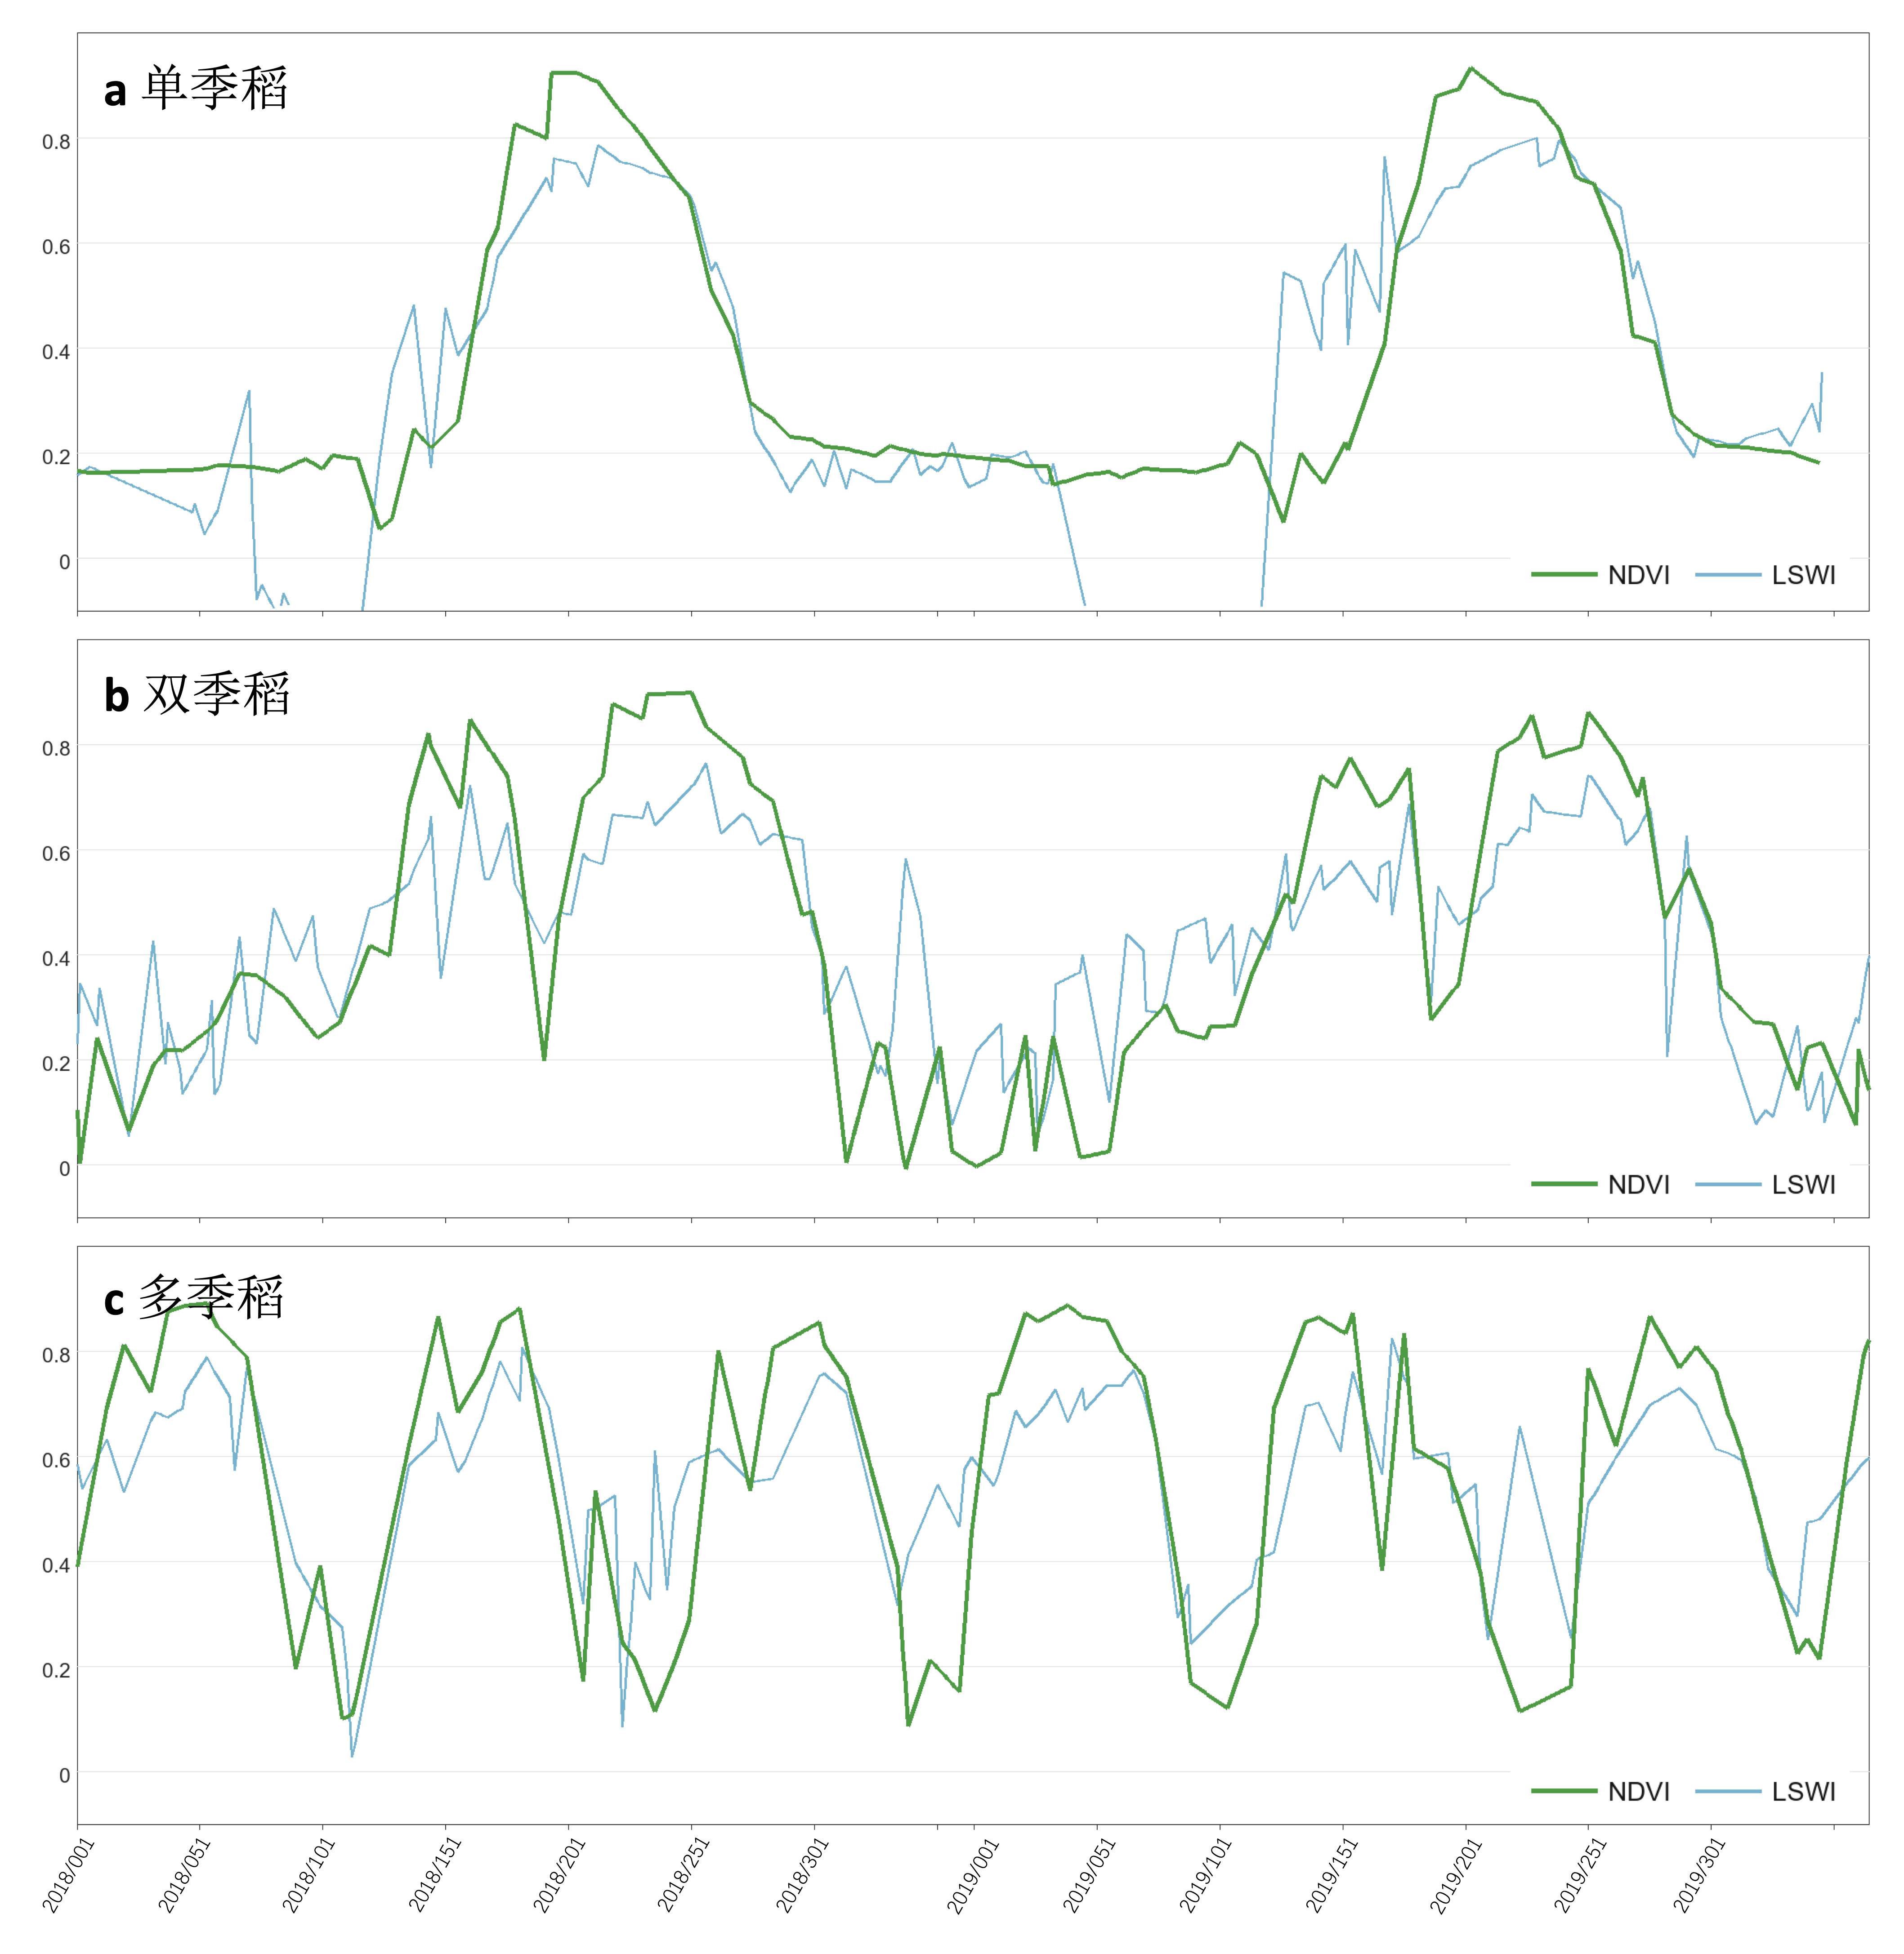
\includegraphics[width=0.95\linewidth]{figure/chapter3/rice_seasons.png}
    \bicaption[不同种植制度下典型水稻像元的 NDVI 和 LSWI 时间序列]{不同种植制度下典型水稻像元的 NDVI 和 LSWI 时间序列：（a）中国东北单季稻样本（45.6937°N，122.9999°E）；（b）中国南方双季稻样本（28.6854°N，112.6057°E）；（c）越南湄公河三角洲三季稻样本（10.3896°N，105.1469°E）。}[Temporal profile of NDVI and LSWI from three typical paddy rice sites with different cropping systems]{Temporal profile of NDVI and LSWI from three typical paddy rice sites with different cropping systems: (a) single paddy rice in Northeast China (45.6937° N, 122.9999° E), (b) double paddy rice in southern China (28.6854° N, 112.6057° E), and (c) triple paddy rice in the Mekong Delta, Vietnam (10.3896° N, 105.1469° E).}
    \label{fig:rice_seasons}
\end{figure}

% 定义研究对象：水稻生长季节
因此，本文将全球水稻动态提取定义为连续日尺度遥感时间序列中的生长季事件识别问题，其核心任务是从像元级 NDVI--LSWI 时间序列中确定水稻生长季的起始、结束及年内发生次数。设像元 \(p\) 具有日尺度 NDVI 序列 \(N_p(t)\) 和 LSWI 序列 \(W_p(t)\)，其识别结果不是单一年度标签，而是一组具有明确时间边界的生长季事件：
\begin{equation}
    \mathcal{E}_p = \{(s_k, e_k)\mid k=1,2,\ldots,n_p\},
    \label{eq:rice_event_set}
\end{equation}
其中，\(s_k\) 和 \(e_k\) 分别表示第 \(k\) 个水稻生长季事件的起始时间（Start of Season, SOS）和结束时间（End of Season, EOS），\(n_p\) 为该像元在给定时间范围内识别出的水稻生长季次数。与年度水稻/非水稻标签相比，式\ref{eq:rice_event_set}直接刻画了同一像元在连续时间轴上的水稻种植过程，使单季、双季、多季以及跨年生长季均可被统一表达。基于水稻生长季的事件集合 \(\mathcal{E}_p\)，年度水稻种植面积、收获面积、复种次数、生长季长度、逐日水稻状态以及环境效应分析所需的真实生长季窗口，均可由像元级生长季事件进一步汇总得到。由此，水稻制图从空间维度上的静态分类转变为时间维度上的事件检测。

% 全球水稻动态提取的算法需求
全球水稻种植制度的高度异质性决定了算法必须具备物候自适应能力。全球水稻播栽期、收获期和种植季次数具有显著区域差异，热带地区水热条件充足，水稻可在全年多个时段播栽，而温带稻区多集中于相对稳定的夏季生长季 \cite{Laborte2017SciData,Mishra2021IJAEO}。如果在全球尺度使用固定月份窗口，南半球稻作可能与北半球窗口错位，热带多季稻可能被遗漏或合并，跨年生长季也可能被自然年边界截断。如果采用固定长度曲线匹配，短季稻会被迫引入无效观测，长季稻则可能丢失关键生育阶段信息。相反，若完全取消物候先验，仅依赖全年曲线匹配，则湿地、水生植被、季节性积水耕地和其他轮作作物可能因局部形态相似而产生较高混淆。

面向上述问题，全球水稻动态提取方法至少需要同时满足三个条件。首先，算法应能够在时间轴上动态搜索候选生长季窗口（SOS 和 EOS），而不是完全依赖区域固定播栽月份，以保证热带多熟区、南半球稻区和作物历资料不足区域仍可被识别。其次，候选生长季窗口应依据实际 NDVI 曲线变化和本地生长季长度约束自适应确定，而不是按统一天数截断，以避免将不同品种、制度和气候区的水稻强行映射到同一时间尺度。再次，算法应能够判断候选生长季窗口内的曲线是否真正对应水稻生长过程，并根据判定结果决定下一轮搜索起点，从而在同一像元内支持单季、双季、多季和跨年水稻生长季的连续识别。上述要求将水稻物候先验、曲线形态判别和时序反馈机制统一到动态水稻生长季事件识别框架中，使方法既具有可解释的农业遥感机理，又具备全球推广所需的时间弹性。

基于上述条件，本研究设计并开发了水稻生长季事件识别框架 MPD\_DTW。该框架由 MPD 模块、DTW 模块和二者之间的反馈机制组成，MPD 模块负责从逐日 NDVI--LSWI 时间序列中搜索候选 SOS 和 EOS，DTW 模块负责比较候选生长季内的 NDVI 曲线与区域标准水稻曲线之间的形态相似性。反馈机制则根据 DTW 判定结果更新下一轮 SOS 搜索起点。由此，MPD 解决"从哪里截取候选曲线"的问题，DTW 解决"截取曲线是否符合水稻生长过程"的问题，反馈机制解决"如何在同一时间轴上连续识别多个季节"的问题。该设计将物候阈值和曲线匹配置于一个闭环搜索框架中。物候检测为曲线匹配提供具有农业意义的候选边界，避免 DTW 在全年复杂曲线中盲目搜索；曲线匹配检验物候候选是否具有完整水稻生长过程，避免单一淹水信号或局部 NDVI 下降造成误判；反馈机制进一步将单次候选判别转化为连续时间轴上的事件序列识别，使算法能够在同一像元内识别多个非重叠生长季。该框架因而兼具基于物候规则方法的可解释性和基于时间序列相似性方法的弹性，是后续构建全球水稻时空动态数据的核心方法基础。

\section{基于生长季事件识别的通用水稻遥感提取框架MPD\_DTW}

\subsection{基于移动物候检测的候选生长季识别}

\label{sec:mpd}

移动物候检测（Moving Phenological Detection, MPD）模块的任务，是在逐像元日尺度遥感时间序列中识别具有水稻物候可能性的候选生长季边界。这里的"移动"并非固定长度滑动窗口，而是沿时间轴连续检查水稻起始期信号：当某一日满足候选 SOS 条件后，算法在该日期之后的本地生长季长度范围内搜索候选 EOS；若该候选 SOS--EOS 片段不能被后续 DTW 模块确认为水稻，则搜索位置继续向后移动。MPD 因而不是一个最终分类器，而是一个带有农业物候约束的候选事件生成器。图\ref{fig:mpd_flowchart}概括了 MPD 模块从日尺度 NDVI--LSWI 序列中检测 SOS 和 EOS 的基本流程。

\begin{figure}[htbp]
    \centering
    
\includegraphics[width=0.85\textwidth]{figure/chapter3/mpd_flowchart.pdf}
    \caption{MPD 模块逐日移动搜索与物候检测流程示意图。}
    \label{fig:mpd_flowchart}
\end{figure}

\subsubsection{输入时序与候选像元约束}

MPD\_DTW 的输入为像元 \(p\) 的日尺度 NDVI 序列 \(N_p(t)\) 和 LSWI 序列 \(W_p(t)\)。在数据预处理阶段，MODIS Terra 与 Aqua 双星 8 d 地表反射率产品（MOD09A1 与 MYD09A1）被用于计算 NDVI 和 LSWI。为降低云雨污染对绿度曲线的影响，NDVI 在每个 8 d 合成窗口内取 Terra 与 Aqua 可用观测中的最大值\cite{Weng2025}；该最大值合成策略能够在不显著损失时间分辨率的前提下，尽可能保留无云观测信息\cite{Zhang2003RSE}。由于水稻移栽期淹水信号持续时间较短，LSWI 保留该窗口内所有可用观测中的水分信息，不进行最大值合成或过度平滑，以避免削弱短时水分峰值\cite{Huang2013RiceUncertainty,Weng2025}。

进入物候检测前，NDVI 日尺度序列进一步采用 41 d 窗口、3 阶多项式的 Savitzky--Golay 滤波进行平滑，以降低残余云、气溶胶、双向反射差异和异常低值对局部导数判断的影响。Savitzky--Golay 滤波通过局部多项式拟合保留曲线峰值宽度与线型特征，在植被指数时间序列重建中具有广泛应用\cite{Chen2004RSE}。记平滑后的 NDVI 为：
\begin{equation}
    \widetilde{N}_p(t)=\mathrm{SG}_{41,3}\{N_p(t)\}.
    \label{eq:sg_ndvi}
\end{equation}
LSWI 序列则采用线性插值获取日尺度值，在 MPD 判定中保留原始水分信号的相对变化，不再施加同等强度的平滑。

为减少非农用地、水体、林地和城市地表对候选事件生成的干扰，MPD 仅在候选耕地像元内运行。本文使用 MCD12Q1 IGBP cropland、GlobeLand30 cultivated land 以及美国 Cropland Data Layer（CDL）等土地覆盖资料构建耕地掩膜：在美国境内以 CDL 聚合结果（耕地比例 $\geq$ 50\%）约束候选像元；其余地区使用 IGBP 耕地与 GlobeLand30 耕地的并集，同样保留耕地比例不低于 50\% 的像元\cite{Weng2025}。对于空间分辨率显著高于 500 m 的参考水稻图（如 10 m 或 30 m），先以 $L \times L$ 扫描窗口筛选空间连续且水稻比例较高的区域，剔除破碎边界像元，再将纯化后的高分辨率水稻图聚合到 500 m MODIS 网格，仅标记水稻比例超过 50\% 的像元为可靠水稻样本\cite{Weng2025}；对于澳大利亚等仅有概率型水稻参考数据的区域，则结合 PhenoRice 算法选取高可信度水稻像元作为标准曲线来源\cite{Boschetti2017RSE}。这一空间约束并不直接判定水稻，而是限定 MPD\_DTW 的搜索域，使后续时序判别集中于可能发生作物种植的像元。

\subsubsection{SOS 的淹水物候依据}

水稻区别于多数旱地作物的关键遥感特征，来自移栽或返青初期浅水层、湿润土壤和稀疏幼苗共同作用形成的水分--植被组合信号。短波红外波段对地表和冠层液态水高度敏感，因此基于近红外和短波红外波段构建的 LSWI 能够表征植被与土壤背景水分变化\cite{Gao1996}。在典型移栽稻田中，早期浅水覆盖增强 LSWI，而绿色植被覆盖度仍较低，NDVI 尚未进入快速上升阶段；随着水稻返青、分蘖和冠层闭合，NDVI 迅速升高并逐渐超过水分信号。Xiao 等在中国南方以及南亚、东南亚的 MODIS 水稻制图研究表明，水稻移栽期 LSWI 接近或高于植被指数的特征能够有效区分水稻与多数旱作物\cite{Xiao2005,Xiao2006}。

基于上述物候机理，候选 SOS 由平滑 NDVI 与日尺度 LSWI 的相对关系触发。对像元 \(p\) 在日期 \(t\) 的候选 SOS 判定为：
\begin{equation}
    W_p(t)+F_z>\widetilde{N}_p(t), \quad
    -1<\widetilde{N}_p(t)<N_{\max}, \quad
    t\in\Omega_{\mathrm{SOS},z},
    \label{eq:sos_condition}
\end{equation}
其中，\(F_z\) 为参数区 \(z\) 的洪水因子，\(N_{\max}=0.5\) 为起始期 NDVI 上限，\(\Omega_{\mathrm{SOS},z}\) 为该参数区允许搜索的候选 SOS 日期集合。\(N_{\max}\) 用于排除已经进入高冠层覆盖阶段的日期，避免将旺盛生长期误判为生长季起点。\(F_z\) 控制水分信号判定的宽松程度：当 \(F_z=0\) 时，只有 LSWI 明显接近或超过 NDVI 的强淹水信号可以触发 SOS；当 \(F_z>0\) 时，弱淹水、混合像元、雨养稻或间歇灌溉稻田中 LSWI 略低于 NDVI 的情形也可能进入候选集合。该判定在实现中通过向量化运算逐日检查，所有满足式\ref{eq:sos_condition} 的日期构成候选 SOS 集合。

\(\Omega_{\mathrm{SOS},z}\) 体现了 MPD 的区域化物候先验。对于中国东北、韩国、日本、欧洲、美国等播栽期相对集中的温带单季稻区，候选 SOS 限定在春末至夏初的 DOY 范围内（如 DOY 121--193）；对于南亚、东南亚、非洲以及中美洲和南美北部等多熟区，作物历在空间和年际间高度异质，\(\Omega_{\mathrm{SOS},z}\) 设置为全年搜索（DOY 1--365）。对巴西南部和澳大利亚等南半球稻区，SOS 窗口位于自然年后部（如 DOY 250--360 或 290--360），EOS 则可能出现在下一年。该设计将已知作物历作为软约束引入候选生成过程，同时避免将全球水稻强行约束到统一播栽月份。

\subsubsection{EOS 的收获物候依据}

候选 EOS 的识别基于水稻成熟收获后绿色生物量下降和 NDVI 低值趋稳的物候特征。水稻从抽穗灌浆进入成熟阶段后，叶片衰老、含绿量下降；收获后地表由高生物量冠层转为残茬、裸土、浅水或翻耕背景，NDVI 通常出现明显下降。与 SOS 侧重水分--植被相对关系不同，EOS 主要依赖 NDVI 曲线的局部衰退特征。对于候选 SOS \(s\)，MPD 仅在本地生长季长度约束内搜索 EOS：
\begin{equation}
    s+T_{1,z}\leq e\leq \min(s+T_{2,z}, E_{\max,z}),
    \label{eq:growing_length}
\end{equation}
其中，\(T_{1,z}\) 和 \(T_{2,z}\) 分别表示参数区 \(z\) 的水稻生长季长度下限和上限，\(E_{\max,z}\) 表示可接受的最晚 EOS 位置，由输入序列末端保留天数决定。若参数区未设置尾部约束，则 \(E_{\max,z}\) 为可用观测序列的最后日期。该长度约束用于排除短期积水、云噪声或非作物扰动造成的不合理短周期事件，同时防止候选季节跨越真实收获期并吞并后续季节。

在式\ref{eq:growing_length}限定的窗口内，候选 EOS 需要同时满足 NDVI 从前一日下降、当前日之后下降速度减弱或趋稳、且 NDVI 已回落至收获期低值范围。具体而言，算法首先计算 NDVI 序列的一阶前向差分 \(\Delta_{-}\widetilde{N}_p(e)=\widetilde{N}_p(e)-\widetilde{N}_p(e-1)\) 和后向差分 \(\Delta_{+}\widetilde{N}_p(e)=\widetilde{N}_p(e)-\widetilde{N}_p(e+1)\)。候选 EOS 需同时满足：
\begin{equation}
    \Delta_{-}\widetilde{N}_p(e)<0,\quad
    \Delta_{+}\widetilde{N}_p(e)<r,\quad
    \widetilde{N}_p(e)\leq N_{\mathrm{eos}},
    \label{eq:eos_condition}
\end{equation}
其中，\(r=0.0025\) 为成熟期下降后趋稳的速率阈值，\(N_{\mathrm{eos}}=0.5\) 为收获期 NDVI 上限。式\ref{eq:eos_condition}并不要求 EOS 是全年 NDVI 的绝对最小值，而是要求其处于候选 SOS 后合理生长季长度范围内，并表现为由高绿度阶段衰退后的近局部低值。若候选 SOS 后不存在满足式\ref{eq:eos_condition}的 EOS，该 SOS 不构成完整候选生长季，算法继续向后搜索新的候选 SOS。实现中，\(\Delta_{-}\) 与 \(\Delta_{+}\) 通过数组移位运算批量计算，所有满足三项条件的日期被一次性提取为候选 EOS 集合。

\subsubsection{候选季节集合生成}

对任一候选 SOS \(s\)，MPD 可能识别出多个满足 EOS 条件的日期。本文将这些候选片段表示为：
\begin{equation}
    \mathcal{C}_p(s)=\{(s,e)\mid e\in\Omega_{\mathrm{EOS}}(s),\ I_{\mathrm{EOS}}(e)=1\},
    \label{eq:candidate_set}
\end{equation}
其中，\(\Omega_{\mathrm{EOS}}(s)\) 为式\ref{eq:growing_length}定义的 EOS 搜索窗口，\(I_{\mathrm{EOS}}(e)=1\) 表示日期 \(e\) 满足式\ref{eq:eos_condition}的收获期判据。MPD 阶段不直接在多个 \(e\) 中确定最终 EOS，而是将候选 SOS--EOS 曲线交由 DTW 模块计算与标准水稻曲线的相似性，并由最小 DTW 距离决定该 SOS 对应的最优 EOS。这样处理避免了仅凭局部 NDVI 极小值确定收获期所导致的不稳定性，使 EOS 同时受到收获物候和完整生长曲线形态的约束。

逐日移动策略的核心价值在于摆脱固定作物历对全球制图的限制。温带单季稻候选 SOS 往往集中于春末夏初，EOS 集中于秋季；热带和亚热带多季稻可在一年内出现多个候选 SOS；南半球和跨年稻作系统则可能在自然年后部起始、次年完成收获。只要 NDVI--LSWI 时间序列中存在符合淹水或返青、冠层发育、成熟收获的连续过程，MPD 模块即可生成候选生长季。与此同时，候选生成并不等同于水稻判定，因为季节性湿地、水生植被、短期积水旱地和部分轮作作物也可能触发类似信号，必须进一步依赖 DTW 对完整生长过程进行判别。

\subsection{基于动态时间规整的水稻生长过程判别}

\label{sec:dtw}

MPD 模块能够给出具有水稻物候可能性的候选 SOS--EOS 片段，但淹水信号和收获后 NDVI 下降并非水稻独有。季节性湿地、洪泛低地、水生植被和部分轮作农田也可能在局部时间段内满足相似的水分与绿度变化条件\cite{Zhan2021}。因此，本文引入动态时间规整（Dynamic Time Warping, DTW）模块，对候选生长季内完整 NDVI 曲线进行形态判别。图\ref{fig:dtw_schematic}展示了 DTW 非线性时间轴弯曲和最优路径匹配的基本原理。

DTW 是一种经典的动态规划时间序列匹配方法，能够在保持时间顺序约束的同时寻找两条序列之间的最优匹配路径\cite{Sakoe1978}。与欧氏距离或逐点相关系数不同，DTW 允许局部时间轴发生非线性拉伸或压缩，因此能够减弱不同生长季长度和物候相位差异对曲线比较的影响\cite{Petitjean2012}。这一特性使 DTW 被广泛用于遥感时间序列的物候匹配、土地覆盖制图和作物类型识别\cite{Maus2016,Belgiu2018}。在本文框架中，DTW 并不在全年曲线上盲目搜索水稻，而是在 MPD 已限定的候选 SOS--EOS 片段中判断该曲线是否具有完整水稻生长过程。

\begin{figure}[htbp]
    \centering
    
\includegraphics[width=0.85\textwidth]{figure/chapter3/dtw_schematic.pdf}
    \caption{DTW 非线性时间轴弯曲与最优路径匹配原理示意图。}
    \label{fig:dtw_schematic}
\end{figure}

\subsubsection{生长季曲线非线性匹配的必要性}

水稻生长过程在曲线形态上具有相对稳定的阶段序列：起始期 NDVI 较低，返青和分蘖期 NDVI 快速上升，抽穗灌浆期维持高值，成熟收获后 NDVI 下降至低值。但这一阶段序列在不同稻作制度和气候区中具有显著时间尺度差异。热带短季稻可能在约三个月内完成一个生长季，温带单季稻可持续五个月以上，双季稻和三季稻中每一季的长度又常短于单季稻\cite{Laborte2017SciData,Mishra2021IJAEO}。若使用固定长度曲线比较，必须对候选曲线进行截断、填充或重采样，容易引入无效观测或丢失关键生育阶段。若仅比较峰值日期或峰值大小，则无法区分完整水稻生长过程与其他具有局部高 NDVI 的作物或湿地植被。

DTW 通过允许曲线局部拉伸，使候选曲线中的返青、旺盛生长和成熟下降阶段能够与标准曲线中相同物候阶段对齐，而不要求它们发生在完全相同的序列位置。换言之，DTW 比较的是曲线的阶段顺序和总体形态，而不是固定日期上的逐点差异。MPD 与 DTW 的结合使方法同时具有物候可解释性和时间弹性：MPD 限定了具有农业意义的候选边界，DTW 则检验该边界内是否存在与水稻一致的完整绿度演化过程。

\subsubsection{标准水稻生长曲线构建}

标准水稻生长曲线是 DTW 判别的参照系，其代表性直接影响全球制图的稳定性。本文未采用单一全球模板，而是根据主要稻区物候差异构建区域化日尺度 NDVI 标准曲线。标准曲线主要来源于第二章所述高分辨率水稻参考图、官方作物图、可靠水稻样本区域和已有高质量水稻产品。对于空间分辨率显著高于 500 m 的参考图，先通过 $L \times L$ 扫描窗口筛选空间连续、纯度较高的水稻区域以剔除破碎边界像元，再将纯化后的高分辨率图聚合到 MODIS 500 m 网格，仅保留水稻比例超过 50\% 的像元，以降低田块边界混合像元对标准曲线的影响；对于澳大利亚等概率型参考资料，则结合 PhenoRice 等已有方法选择高可信水稻样本\cite{Boschetti2017RSE,Weng2025}。

区域化标准曲线构建遵循三个原则。第一，模板应覆盖从移栽或返青到成熟收获的完整水稻生长过程，而不是仅刻画峰值附近片段。第二，模板长度应与本地水稻生长季长度相协调，使 DTW 在合理生物学时间尺度内进行弹性匹配。第三，模板应尽量来自高纯度、空间连续的水稻像元，以减少非水稻地物和混合像元对曲线形态的污染。最终参数体系中使用的主要模板包括中国东北（长度约 170 d）、韩国日本（约 160 d）、中国东南（约 140 d）、南亚与东南亚（约 130 d）、美国（约 160 d）、巴西及南美南部（约 160 d）、欧洲（约 160 d）、马达加斯加（约 130 d）和澳大利亚（约 160 d）等参数区。区域模板并不削弱方法的统一性；相反，它使同一 MPD\_DTW 逻辑能够承认不同稻区真实存在的生长季长度、峰值位置和成熟衰退速度差异。

\subsubsection{曲线相似性度量与水稻判定}

设 MPD 生成的候选生长季 NDVI 曲线为 \(A_{s:e}=(a_1,a_2,\ldots,a_m)\)，参数区 \(z\) 的标准水稻曲线集合为 \(\mathcal{R}_{z}=\{R_q\}\)，其中 \(R_q=(r_1,r_2,\ldots,r_n)\)。对任一候选曲线和标准曲线，DTW 构建 \(m\times n\) 的累计距离矩阵，并按如下递推式计算最优匹配代价：
\begin{equation}
    D(i,j)=|a_i-r_j|+\min\{D(i-1,j),D(i,j-1),D(i-1,j-1)\},
    \label{eq:dtw}
\end{equation}
其中，\(|a_i-r_j|\) 为两个时间点 NDVI 值的局部绝对差异，三种转移方向分别对应候选曲线拉伸、标准曲线拉伸和二者同步推进。递推矩阵的边界以起点匹配为初始条件，并通过累计代价保证匹配路径在时间顺序上单调前进。本文采用 symmetric1 步模式，即允许对角、水平和垂直三种等权重转移，该模式在遥感时间序列匹配中具有良好平衡性\cite{Sakoe1978,Petitjean2012}。最终距离 \(D(m,n)\) 表示候选曲线与标准曲线之间的总体不相似度。

若参数区包含多条标准曲线，则以候选曲线到所有标准曲线的最小 DTW 距离作为该候选季节的相似性度量：
\begin{equation}
    d_z(s,e)=\min_{R_q\in\mathcal{R}_{z}}D(A_{s:e},R_q).
    \label{eq:min_dtw}
\end{equation}
对于同一候选 SOS \(s\)，若存在多个候选 EOS，则先选择 DTW 距离最小的 EOS：
\begin{equation}
    e^{*}(s)=\arg\min_{e\in\Omega_{\mathrm{EOS}}(s)} d_z(s,e).
    \label{eq:best_eos}
\end{equation}
给定参数区 DTW 阈值 \(\theta_z\)，候选生长季的水稻判定为：
\begin{equation}
    y(s,e^{*})=
    \left\{
    \begin{array}{ll}
        1, & d_z(s,e^{*})<\theta_z,\\
        0, & d_z(s,e^{*})\geq\theta_z.
    \end{array}
    \right.
    \label{eq:dtw_threshold}
\end{equation}

DTW 距离越小，说明候选曲线在低值起始、快速增绿、峰值维持和成熟下降等方面越接近区域标准水稻物候。需要强调的是，DTW 距离不是分类概率，而是候选曲线与标准生长过程之间的连续不相似性度量。实际制图中同时保存 SOS、EOS 和最小 DTW 距离，以支持阈值判定、参数调整、面积一致性检查和不确定性分析。对于单季稻参数区，全年候选季节中 DTW 距离最小的 SOS--EOS 片段被记录为该像元的最可能水稻季，最终水稻面积由 \(\theta_z\) 判定生成；对于多季稻参数区，算法沿时间轴记录所有满足阈值条件的非重叠季节，并以多波段栅格存储多个 SOS、EOS 和 DTW 距离。

\subsection{水稻生长季事件的连续识别机制}

\label{sec:feedback}

MPD 与 DTW 的反馈机制是 MPD\_DTW 区别于普通物候阈值法或普通曲线匹配法的关键。物候检测提供候选事件，DTW 提供水稻身份判别，而反馈机制决定时间轴如何继续移动。若每次候选检测后简单跳过整个候选窗口，真实水稻季可能因前一个非水稻候选事件而被漏检；若每次只向后移动一日，已确认水稻季内部又可能被重复检测，尤其在长季稻或多季稻衔接区形成重叠季节。图\ref{fig:mpd_dtw_feedback}展示了 MPD 与 DTW 闭环协同的连续识别流程。

\begin{figure}[htbp]
    \centering
    
\includegraphics[width=0.9\textwidth]{figure/chapter3/mpd_dtw_feedback.pdf}
    \caption{MPD\_DTW 反馈机制流程图。}
    \label{fig:mpd_dtw_feedback}
\end{figure}

设当前候选 SOS 为 \(s\)，经 MPD 和 DTW 后得到最优候选季节 \((s,e^{*})\) 及其距离 \(d_z(s,e^{*})\)。若 \(d_z(s,e^{*})<\theta_z\)，则该片段被确认为一次水稻生长季，下一轮 SOS 搜索从该季节 EOS 之后开始：
\begin{equation}
    t_{\mathrm{next}}=e^{*}+1,\quad \mathrm{if}\ d_z(s,e^{*})<\theta_z.
    \label{eq:positive_feedback}
\end{equation}
这一正向反馈保证已确认的水稻季不会被重复识别，并确保同一像元内相邻水稻季在时间上不重叠。对于双季稻和多季稻，前一季收获后算法继续搜索后续候选 SOS；若后续再次出现满足 SOS、EOS 和 DTW 条件的片段，则被记录为第二季或第三季。多季稻识别还读取上一年的最晚 EOS，用于约束当年候选 SOS 必须晚于上一季 EOS，从而避免跨年季节在相邻年份之间重复计数。

若 \(d_z(s,e^{*})\geq\theta_z\)，则当前候选片段虽具有一定水分和绿度变化特征，但整体曲线形态不符合区域水稻标准物候。此时算法不跳至 \(e^{*}+1\)，因为真实水稻季可能在当前候选 SOS 之后不久才开始。MPD\_DTW 因而采用负向反馈，将下一轮搜索位置设为当前 SOS 之后：
\begin{equation}
    t_{\mathrm{next}}=s+1,\quad \mathrm{if}\ d_z(s,e^{*})\geq\theta_z.
    \label{eq:negative_feedback}
\end{equation}
在逐日候选集合已经预先筛选的实现中，负向反馈表现为不更新上一季 EOS 约束，并继续检查后续候选 SOS。该策略在排除当前非水稻候选事件后仍保留精细搜索能力，可降低短期积水、湿地植被或噪声触发候选 SOS 后造成真实水稻季漏检的风险。

\subsubsection{单季稻与多季稻的差异化处理}

全球稻作制度的空间差异要求 MPD\_DTW 在算法实现层面区分单季模式与多季模式。单季模式面向温带单季稻区（如中国东北、韩国日本、美国、欧洲、巴西及澳大利亚），其特点是同一像元在一年内通常仅出现一个完整水稻生长季。在该模式下，算法遍历全年候选 SOS，对所有候选片段计算最优 EOS 及 DTW 距离，最终仅保留距离最小的 SOS--EOS 组合作为该像元当年的最可能水稻季。若最小距离低于 \(\theta_z\)，则该像元标记为水稻；否则标记为非水稻。输出以单波段栅格形式存储 SOS、EOS 和 DTW 距离。

多季模式面向亚热带双季稻区和热带多季稻区（如中国东南、南亚东南亚、非洲、马达加斯加及中美洲）。在该模式下，算法沿时间轴顺序扫描候选 SOS，每当确认一个水稻季（\(d<\theta_z\)），立即将搜索起点移至该季 EOS 之后，继续检测后续季节。对于跨年参数区（除中国东南等部分双季稻区外），输入时间序列读取下一年观测，使当年后期播栽的 SOS 能够在下一年数据中完成 EOS 搜索。多季模式的输出采用多波段栅格，波段按季节时间从后向前组织：第一波段记录当年最晚季节，后续波段依次记录更早季节。每个波段存储 SOS 或 EOS 的 DOY 值，DTW 距离则乘以 100 后以整型存储以保留两位小数。这种编码方式既压缩了存储空间，又保留了像元级多季信息的完整可追溯性。

\subsubsection{预制图与阈值分层校正策略}

多季稻区物候复杂、国家间种植面积差异显著，统一阈值难以同时满足所有国家的面积一致性。为此，本文对多季稻参数区实施"预制图--阈值校正--二次制图"的分层策略。

预制图（pre-mapping）阶段，多季稻参数区首先以相对宽松的 SOS 搜索窗口（DOY 1--282）和基础阈值 \(\theta_z\) 运行 MPD\_DTW，获取全年最小 DTW 距离对应的候选季节。该阶段目的是尽可能不遗漏潜在水稻季，即使部分非水稻像元也被赋予最小距离值。预制图输出包含所有候选像元的 SOS、EOS 和距离值，为后续国家尺度阈值调整提供连续的距离分布。

阈值校正阶段，对于具有可靠 FAO 统计面积的国家，本文以国家边界为空间单元，以预制图输出的距离栅格为基础，通过迭代调整阈值使遥感制图收获面积与 FAO 统计收获面积的相对误差控制在 10\% 以内。具体而言，设某国某年统计面积为 \(A_{\mathrm{stat}}\)，预制图结果中该国耕地范围内所有候选像元的最小距离值为 \(d_{\min}\)。若基础阈值对应的制图面积 \(A_{\mathrm{base}}<A_{\mathrm{stat}}\)，则逐步放宽阈值；若 \(A_{\mathrm{base}}>A_{\mathrm{stat}}\)，则逐步收紧阈值。调整步长初始为 0.1，当面积偏差超过统计面积 10 倍时采用二分法加速收敛。最终得到该国该年的优化阈值 \(\theta_{\mathrm{country}}\)。对于无统计资料或统计可靠性较低的国家，则保留参数区基础阈值。

二次制图（second mapping）阶段，以校正后的国家阈值重新运行 MPD\_DTW。此时 SOS 搜索窗口恢复为参数区全年范围，但仅对预制图阶段已识别为潜在水稻的像元进行二次判别，以减少计算量。若某国校正阈值显著高于基础阈值（差值超过 0.1），表明预制图可能漏检了部分弱信号水稻季，此时算法自动放宽洪水因子至 0.15 并将 NDVI 上限提高至 0.6，以增强 SOS 召回能力，避免因阈值升高而遗漏真实水稻季。二次制图结果即为该国的最终水稻生长季产品。

\subsubsection{跨年处理与年际衔接}

跨年处理是该流程面向全球推广的重要环节。澳大利亚、巴西等南半球或可能跨年的单季稻参数区读取下一年观测，使自然年后部出现的 SOS 能够在下一年数据中完成 EOS 搜索；南亚、东南亚、非洲及美洲热带多季稻区也可读取下一年观测，以识别当年播栽、次年收获的季节。具体实现中，对于需跨年处理的参数区，输入时间序列由当年全年日观测与下一年前期观测拼接而成，总长度视参数区需要而定（通常为当年日数加次年 85--185 d）。

年际衔接通过上年最晚成熟日约束实现。多季模式下，算法读取上一年输出中最晚季节的 EOS（以 DOY 表示，若跨年则转换为相对于当年起始日的索引），当前年份的候选 SOS 必须严格晚于该索引，从而防止同一跨年季节在相邻两年被重复计数。对于起始年（2000 年）或上一年无水稻的像元，该约束自动失效，当年从序列起点开始搜索。由此，GlobalRice500 不仅提供年度水稻空间分布，还保留像元级水稻生长季事件序列，为收获面积统计、复种强度估算和生长季 LST 效应分析提供一致的时间边界。

\subsection{MPD\_DTW参数优选}

\label{sec:sensitivity}

MPD\_DTW 的参数并非纯经验设定，而是由水稻物候机理、参考数据质量、区域种植制度和面积统计约束共同确定。关键参数包括洪水因子 \(F_z\)、SOS 阶段 NDVI 上限 \(N_{\max}\)、候选 SOS 搜索窗口 \(\Omega_{\mathrm{SOS},z}\)、生长季长度约束 \(T_{1,z}\)--\(T_{2,z}\)、EOS 趋稳速率阈值 \(r\)、最晚 EOS 尾部约束、DTW 距离阈值 \(\theta_z\) 以及区域标准水稻曲线。它们分别控制候选 SOS 的召回能力、候选 EOS 的生物学合理性、曲线匹配判定的保守程度，以及全球不同稻作系统的物候差异表达。

\begin{figure}[htbp]
    \centering
    
\includegraphics[width=0.9\textwidth]{figure/chapter3/sensitivity_analysis.pdf}
    \caption{关键参数敏感性分析结果。}
    \label{fig:sensitivity_analysis}
\end{figure}

\subsubsection{参数调优的参考样本体系}

参数调优首先依赖参考水稻图和候选耕地掩膜构建正负样本。正样本来自高纯度水稻像元，即参考水稻比例达到设定阈值且位于候选耕地范围内的像元；负样本来自同一耕地掩膜内的非水稻像元。对于高分辨率参考图，先通过空间连续性扫描和 50\% 水稻比例筛选降低破碎边界像元影响；对于参考资料较弱或概率型资料，则选择高可信水稻像元参与模板和参数确定。正负样本均在参数区、年份和 MODIS tile 层面组织，使参数调优尽量覆盖区域内主要水稻物候类型和非水稻混淆背景。

训练样本的数量与比例直接影响参数估计的稳健性。本文在调参时控制正负样本比例（negative-positive ratio, np\_ratio），使负样本数量不超过正样本的指定倍数，避免因负样本过多而低估召回率。对于样本充足的参数区，训练集按一定比例（通常为 10\%--30\%）随机抽取，剩余样本用于独立验证；对于样本稀少的区域，则采用全部样本参与调参。每个参数区的训练像元数、正负比例和年份覆盖均在调参日志中记录，以保证参数确定过程的可追溯性。

在调参过程中，洪水因子 \(F_z\) 与 DTW 阈值 \(\theta_z\) 通过网格搜索联合评估。对每组候选参数，算法在参考样本上计算真阳性（TP）、假阴性（FN）、假阳性（FP）和真阴性（TN），并进一步计算生产者精度（PA）、用户精度（UA）、总体精度（OA）和 F1 分数：
\begin{equation}
    \mathrm{PA}=\frac{\mathrm{TP}}{\mathrm{TP}+\mathrm{FN}},\quad
    \mathrm{UA}=\frac{\mathrm{TP}}{\mathrm{TP}+\mathrm{FP}},\quad
    \mathrm{OA}=\frac{\mathrm{TP}+\mathrm{TN}}{\mathrm{TP}+\mathrm{FN}+\mathrm{FP}+\mathrm{TN}},
    \label{eq:accuracy_metrics_1}
\end{equation}
\begin{equation}
    \mathrm{F1}=\frac{2\times\mathrm{UA}\times\mathrm{PA}}{\mathrm{UA}+\mathrm{PA}}.
    \label{eq:accuracy_metrics_2}
\end{equation}
参数选择并不单纯追求某一指标最大化，而是在 F1、OA、UA 与 PA 的平衡关系、国家或次国家统计面积一致性、典型区域物候合理性之间综合确定。尤其在全球制图中，过低阈值可能产生较高 UA 但漏检弱信号水稻，过高阈值则可能提高 PA 但引入湿地或其他作物错分，因此需要结合参考区精度和统计面积共同约束。

\subsubsection{洪水因子与 SOS 判定严格程度}

洪水因子 \(F_z\) 控制式\ref{eq:sos_condition}中 LSWI 与 NDVI 相对关系的宽松程度，是 MPD 模块中最直接影响候选 SOS 数量的参数。理论上，移栽稻田在浅水覆盖和低植被覆盖阶段常表现为 LSWI 接近或高于 NDVI；但在 500 m 混合像元、弱灌溉、雨养稻、间歇灌溉或残余噪声影响下，LSWI 可能略低于 NDVI。若 \(F_z\) 过小（如 \(F_z=0\)），算法只接受强淹水信号，容易漏检弱淹水稻区和混合像元中的真实水稻；若 \(F_z\) 过大（如 \(F_z\geq0.15\)），季节性湿地、短期积水旱地或非水稻水生植被也可能进入候选集合，增加后续 DTW 判别负担和潜在错分风险。

因此，本文采用区域化 \(F_z\) 设置。温带单季稻区和机械化灌溉稻区（如中国东北、韩国日本）通常具有较稳定的播栽期和较清晰的水分信号，\(F_z\) 取较低值（0--0.04）；热带多熟区、雨养稻区或参考样本显示淹水信号较弱的区域（如南亚东南亚、非洲、中美洲），则适当提高 \(F_z\)（0.06--0.09）以保持候选生成的召回能力。由于 DTW 会进一步判别完整 NDVI 生长过程，MPD 阶段的 \(F_z\) 更强调不遗漏潜在水稻季，而非单独完成最终分类。换言之，\(F_z\) 的合理取值应服务于候选生成，其误检风险由 DTW 阈值、耕地掩膜、区域参数和反馈机制共同控制。

\subsubsection{生长季长度约束与 EOS 本地化}

生长季长度约束 \(T_{1,z}\)--\(T_{2,z}\) 是连接 SOS 与 EOS 的关键参数。其作用不是规定所有水稻必须具有相同生长周期，而是在全球差异背景下排除生物学上明显不合理的候选事件。若 \(T_{1,z}\) 过短，短期积水、云噪声或非水稻植被短暂增绿可能被误识别为完整生长季；若 \(T_{2,z}\) 过长，一个候选 SOS 可能跨越真实收获期并吞并后续种植季，尤其在双季稻和热带多季稻区造成季节粘连。

本文依据区域稻作制度、参考样本物候曲线和最终制图参数，为不同参数区采用不同 \(T_{1,z}\)--\(T_{2,z}\) 组合。温带单季稻区通常采用较长的生长季约束，如中国东北、韩国日本、欧洲、美国、澳大利亚等区域多采用 130--200 d 或 140--200 d 的范围；亚热带双季稻和热带多季稻区则采用更短或更弹性的范围（85--175 d 或 90--195 d），以适应多季种植和季节差异。最晚 EOS 尾部约束用于防止在输入序列末端识别缺少后续观测支撑的候选季节。例如，部分温带单季稻区保留约 30 d 尾部观测，中国东南保留约 20 d，澳大利亚因南半球生长季跨年和输入序列结构特殊设置 185 d 的尾部约束。未设置该约束的参数区，则由可用输入序列、\(T_{1,z}\)--\(T_{2,z}\) 和 NDVI 下降条件共同确定 EOS。

\subsubsection{DTW 阈值与区域化参数体系}

DTW 阈值 \(\theta_z\) 决定候选生长季被确认为水稻的严格程度。阈值偏低时，只有与标准水稻曲线高度相似的候选季节被接受，通常有利于提高 UA，但可能漏检弱信号水稻、混合像元和特殊管理制度水稻；阈值偏高时，水稻召回能力可能提高，但与水稻曲线相似的非水稻湿地或其他作物也更容易被纳入。因此，\(\theta_z\) 的选择需要在像元级分类精度、国家尺度面积一致性和区域物候差异之间取得平衡。

本文先基于参考水稻区域通过网格搜索确定基础阈值，使参考区的 F1 或 OA 达到较优水平；再结合 FAO 或次国家统计面积进行年度和国家尺度检查，对必要区域进行阈值校正，使遥感收获面积与统计收获面积在合理误差范围内保持一致\cite{Weng2025}。表\ref{tab:mpd_dtw_parameters}概括了最终制图中主要参数区的基础参数。表中"全年"表示候选 SOS 不限定固定 DOY 窗口，而是在输入日尺度序列中完整移动搜索；"未设"表示未显式设置距离输入序列末端的最晚 EOS 尾部约束。需要注意的是，该表反映 MPD\_DTW 的基础参数体系，最终数据产品构建中部分国家和年份还会结合统计面积与参考区域验证进行阈值校正，这一数据产品层面的校正将在第四章展开。

\begin{table}[htbp]
    \centering
    \bicaption{MPD\_DTW 主要参数区基础参数设置}{Parameter settings for main MPD\_DTW parameter zones}
    \label{tab:mpd_dtw_parameters}
    \begin{tabular}{@{}p{0.2\textwidth}p{0.08\textwidth}p{0.07\textwidth}p{0.13\textwidth}p{0.07\textwidth}p{0.14\textwidth}p{0.12\textwidth}@{}}
        \toprule
        参数区 & 模式 & \(\theta_z\) & SOS 窗口（DOY） & \(F_z\) & \(T_1\)--\(T_2\)（d） & EOS 尾部约束（d） \\
        \midrule
        中国东北及相近温带区 & 单季 & 4.1 & 121--193 & 0.00 & 130--200 & 30 \\
        韩国、日本 & 单季 & 3.5 & 121--193 & 0.00 & 130--200 & 30 \\
        中国东南 & 多季 & 3.7 & 80--210 & 0.02 & 90--195 & 20 \\
        南亚与东南亚 & 多季 & 2.9 & 全年 & 0.09 & 85--175 & 未设 \\
        中美洲及南美北部 & 多季 & 2.9 & 全年 & 0.09 & 85--175 & 未设 \\
        美国 & 单季 & 7.7 & 111--193 & 0.04 & 120--200 & 30 \\
        巴西及南美南部 & 单季 & 5.0 & 250--360 & 0.08 & 130--200 & 未设 \\
        欧洲稻区 & 单季 & 3.3 & 111--183 & 0.08 & 140--200 & 30 \\
        非洲稻区 & 多季 & 5.2 & 全年 & 0.06 & 90--180 & 未设 \\
        澳大利亚 & 单季 & 2.7 & 290--360 & 0.02 & 140--200 & 185 \\
        \bottomrule
    \end{tabular}
\end{table}

\subsubsection{敏感性分析的解释框架}

参数敏感性分析的目的不是寻找一个可在全球所有地区机械套用的单一最优数值，而是检验 MPD\_DTW 框架在合理参数扰动下是否保持稳定。图\ref{fig:sensitivity_analysis}从候选 SOS、SOS/EOS 时序、DTW 阈值和面积响应等方面展示了关键参数变化对结果的影响。对 \(F_z\) 的敏感性分析重点关注候选 SOS 数量、弱淹水稻区召回率和湿地错分风险；对 \(T_{1,z}\)--\(T_{2,z}\) 的敏感性分析重点关注季节粘连、短周期噪声和单季/多季判别；对 \(\theta_z\) 的敏感性分析则同时评估像元级 OA、UA、PA、F1 以及国家尺度面积一致性。

从方法逻辑上看，MPD\_DTW 的稳健性来自多重约束的叠加。SOS 由水分--植被相对关系筛选，EOS 由生长季长度、NDVI 下降和低值趋稳共同限定，DTW 由完整曲线形态进行二次判别，耕地掩膜和区域参数进一步限制空间和物候搜索范围。因此，即使某一参数存在局部不确定性，其影响也会被其他模块部分缓冲。若轻微参数扰动导致全球面积或典型区精度剧烈波动，说明方法过度依赖局部阈值；若结果在合理扰动范围内保持稳定，则表明主要判别信息来自水稻时序过程本身，而非偶然阈值。第四章将从高分辨率参考图验证和 FAO 统计验证两个层面进一步检验本章参数体系的可靠性。

\section{全球水稻面积时空数据基座构建}

本章系统介绍 GlobalRice500 全球水稻遥感数据集的构建流程与多维度精度验证。该数据集基于 MPD\_DTW 方法，利用 2000--2023 年超过 40 TB 的卫星影像，构建了 2001--2022 年、日尺度、500 m 分辨率的全球水稻空间分布产品。本章从空间验证、统计验证、产品对比和不确定性四个维度论证 GlobalRice500 的可信度，为后续全球水稻时空格局及气候效应分析奠定数据基础。

本研究的验证数据主要包括两类：一类是用于参数选择和空间精度评价的高分辨率水稻图或人工解译数据，另一类是用于宏观面积一致性检验的统计数据。二者分别对应不同尺度的可靠性问题。高分辨率参考图能够检验像元级空间识别是否准确，统计数据则能够检验国家或次国家尺度的年度水稻收获面积是否与官方农业统计相一致。由于 GlobalRice500 需要同时提供空间分布、生长季起止和年度收获面积信息，多类型参考数据可以更充分地评价其可靠性。

\subsection{构建流程}

\subsubsection{全球影像预处理与分块策略}

本节说明原始 MODIS 影像的获取、筛选、拼接及全球分块（tile）处理策略。由于数据量巨大，需采用分布式或分块并行处理框架，对全球陆地表面进行规则格网划分，确保计算可扩展性和内存可控性。MODIS植被指数产品经过严格的辐射定标和大气校正，为长时序分析提供了稳定的数据基础\cite{Huete2002}。同时需说明云掩膜、质量控制及时间序列缺值处理的基本策略，包括Savitzky-Golay滤波平滑和时间序列重建技术，旨在最大程度恢复植被指数的物候信息。

\begin{figure}[htbp]
    \centering
    
\includegraphics[width=0.9\textwidth]{figure/chapter4/globalrice500_workflow.pdf}
    \caption{GlobalRice500数据集构建总体流程图。}
    \label{fig:globalrice500_workflow}
\end{figure}

\subsubsection{逐像元水稻识别算法}

本节阐述基于 MPD\_DTW 的逐像元水稻识别流程。重点说明如何利用 NDVI 和 LSWI 双指数时间序列刻画水稻特有的淹水—移栽—生长—成熟物候特征\cite{Xiao2006,Gao1996}，以及 DTW 距离度量在匹配标准物候模板时的优势\cite{Petitjean2012}。MPD模块通过逐日移动检测自适应地确定每个潜在生长季的起止时间，DTW模块则通过柔性时间轴弯曲对候选曲线与标准水稻模板进行相似性度量。该流程对单季稻、双季稻和多季稻具有良好的区分能力，无需预先输入区域种植制度先验信息\cite{Dong2016}。

\subsubsection{逐日生长季记录与年度汇总}

本节介绍在识别水稻像元的基础上，如何进一步记录每个像元的逐日生长季信息，包括移栽期（SOS）和成熟期（EOS）。随后说明将逐日识别结果按水文年或日历年汇总，生成年度水稻种植面积图层的方法。需提及面积计算中像元面积随纬度变化的校正处理，确保不同纬度区域面积统计的准确性和可比性。这种逐日记录机制使GlobalRice500区别于传统仅提供年度分布图的水稻产品，为物候—气候耦合研究提供了前所未有的数据支撑。

\subsubsection{产品格式与变量定义}

本节描述 GlobalRice500 数据集的存储格式（GeoTIFF）、坐标参考系统（WGS84）、时间覆盖范围（2001--2022 年）、空间分辨率（500 m）及包含的变量。主要变量包括：年度水稻种植空间分布图层（二值标识）、生长季起始日（SOS）、生长季结束日（EOS）、以及逐日水稻种植状态图层等。产品元数据记录了数据来源、处理版本、质量控制标志及不确定性等级等关键信息，便于用户进行后续分析和不确定性评估。

\subsection{验证与评价}

\subsubsection{基于高分辨率水稻图的空间验证}

\subsubsection{验证方法与精度指标}

本节说明空间验证的总体方案：以高分辨率参考水稻图（如基于 Sentinel-2、Landsat 或目视解译的 10--30 m 产品）为真值，通过上采样或聚合至 500 m 分辨率后，计算混淆矩阵、总体精度（OA）、用户精度（UA）、生产者精度（PA）和 F1 分数\cite{Han2021,Zhang2017STOTEN}。需说明验证样本区的选取原则，即兼顾不同大洲、气候带、种植制度和景观破碎度。基于高分辨率参考图的空间验证是评估中分辨率遥感产品精度的可靠方法，已在多项水稻制图研究中得到广泛应用\cite{Dong2016}。

\begin{figure}[htbp]
    \centering
    
\includegraphics[width=0.9\textwidth]{figure/chapter4/validation_sites_map.pdf}
    \caption{全球九个验证区的空间分布示意图。}
    \label{fig:validation_sites_map}
\end{figure}

\subsubsection{中国东北典型区验证}

中国东北是世界三大黑土带之一，也是我国最重要的单季稻产区，稻田连片分布、机械化程度高\cite{Han2021}。本节以2018年目视解译水稻分布图为参考，展示该区域 GlobalRice500 与高分辨率参考图的对比结果。验证结果显示，GlobalRice500在该区域具有极高的识别精度，总体精度（OA）达到97.21\%，F1分数为90.51\%，用户精度（UA）为90.59\%，生产者精度（PA）为90.43\%。尽管总体精度极高，但在稻田边界像元处仍存在一定程度的混淆，这主要源于500 m分辨率下稻田与道路、村落等非耕地地物的混合效应。

\subsubsection{中国东南典型区验证}

中国东南地区（如长江中下游、珠江三角洲）水稻种植制度复杂，单季稻、双季稻并存，且稻田与水体、城镇交错分布\cite{Zhang2017STOTEN,Zhang2020NatCommun}。本节以 NESEA-Rice10（2017--2019）产品为参考数据进行验证。结果显示，GlobalRice500 在该区域的总体精度（OA）为88.85\%，F1分数为85.19\%，用户精度（UA）为85.63\%，生产者精度（PA）为84.76\%，略低于其他区域。本节分析混合像元和景观破碎化对该区域精度的影响，特别是在双季稻区，两季之间的休闲期较短，对MPD的季间区分能力提出了更高要求。

\subsubsection{东南亚典型区验证}

东南亚（如越南湄公河三角洲、泰国中部平原、印度尼西亚爪哇岛）是全球水稻种植最集中的区域之一，雨养稻与灌溉稻并存，生长季多样\cite{Xiao2006}。本节以 Sun et al. 2023（ESSD）和 NESEA-Rice10 产品为参考进行验证。结果显示，GlobalRice500 在该区域的总体精度（OA）为95.40\%，F1分数为89.82\%，用户精度（UA）为89.86\%，生产者精度（PA）为89.78\%。本节进一步讨论热带多云地区影像质量对识别精度的潜在影响。尽管预处理阶段采用了时间序列重建技术，部分云雨密集区的物候信号仍可能存在一定扭曲。

\subsubsection{南亚典型区验证}

南亚（如印度恒河平原、孟加拉国）是全球水稻面积最大的区域，种植制度从单季到三季稻不等\cite{Zhang2017STOTEN,Zhang2020NatCommun}。本节展示该区域验证结果，重点讨论大面积连片稻田区域的高精度特征。在孟加拉国等强降雨养稻交错区域，以及印度部分田块破碎的丘陵稻区，精度呈现一定的空间异质性。

\subsubsection{美国与巴西典型区验证}

美国和巴西分别是美洲水稻生产的重要代表，种植区域相对集中，机械化程度高。本节分别以美国 CDL（Cropland Data Layer，2008--2022）和巴西 Conab Mapeamentos Agricolas（2019）为参考数据进行验证。结果显示，美国典型区的总体精度（OA）为95.80\%，F1分数为80.73\%，用户精度（UA）为80.66\%，生产者精度（PA）为80.80\%；巴西 Rio Grande do Sul 典型区的总体精度（OA）为94.34\%，F1分数为83.13\%，用户精度（UA）为83.26\%，生产者精度（PA）为83.01\%。本节说明 GlobalRice500 在美洲地区的适用性：美国南部稻区以灌溉单季稻为主，物候信号清晰；巴西则拥有大面积的热带雨养稻和灌溉稻，种植时间跨度较大。算法在这两种不同气候背景下均表现出稳健的性能。

\subsubsection{欧洲与非洲典型区验证}

本节展示意大利（Lombardia，欧洲典型水稻区）和马达加斯加（非洲独特水稻区）的验证结果，并补充澳大利亚典型区的验证概况。意大利参考数据为 Carta Uso Agricolo（2014--2019），马达加斯加参考数据为2019年目视解译结果，澳大利亚参考数据为2010年全国土地利用数据（National scale land use data）。验证结果显示，意大利 Lombardia 地区的总体精度（OA）为94.42\%，F1分数为81.54\%，用户精度（UA）为81.75\%，生产者精度（PA）为81.34\%；马达加斯加地区的总体精度（OA）为95.32\%，F1分数为93.88\%，用户精度（UA）为93.88\%，生产者精度（PA）为93.88\%；澳大利亚地区的总体精度（OA）高达99.60\%，F1分数为79.27\%，用户精度（UA）为80.10\%，生产者精度（PA）为78.46\%。意大利稻田分布集中，而马达加斯加梯田景观独特，二者对算法的迁移能力提出了不同挑战\cite{Onojeghuo2018}。GlobalRice500 在意大利稻区和马达加斯加均表现优异，在澳大利亚因稻田面积占比较低，总体精度虽高，但F1分数相对有限。

\subsubsection{全球空间验证综合评述}

本节汇总全球九个典型验证区域的精度结果（表\ref{tab:validation_summary}），分析空间分布规律：哪些区域精度高、哪些区域存在系统性漏分或错分，以及景观破碎度、种植制度复杂度与精度之间的关系。

\begin{table}[htbp]
    \centering
    \caption{GlobalRice500全球典型验证区空间精度汇总。}
    \label{tab:validation_summary}
    \small
    \begin{tabular}{lccccp{5.2cm}}
        \toprule
        验证区域 & OA (\%) & F1 (\%) & UA (\%) & PA (\%) & 参考数据来源 \\
        \midrule
        中国东北 & 97.21 & 90.51 & 90.59 & 90.43 & 目视解译，2018 \\
        中国东南 & 88.85 & 85.19 & 85.63 & 84.76 & NESEA-Rice10, 2017--2019 \\
        朝鲜半岛与日本 & 93.45 & 81.57 & 81.85 & 81.29 & Jo et al. 2023; Inoue et al. 2020; Carrasco et al. 2022 \\
        东南亚 & 95.40 & 89.82 & 89.86 & 89.78 & Sun et al. 2023; NESEA-Rice10 \\
        澳大利亚 & 99.60 & 79.27 & 80.10 & 78.46 & National land use data, 2010 \\
        马达加斯加 & 95.32 & 93.88 & 93.88 & 93.88 & 目视解译，2019 \\
        意大利（Lombardia） & 94.42 & 81.54 & 81.75 & 81.34 & Carta Uso Agricolo, 2014--2019 \\
        美国 & 95.80 & 80.73 & 80.66 & 80.80 & CDL, 2008--2022 \\
        巴西（Rio Grande do Sul） & 94.34 & 83.13 & 83.26 & 83.01 & Conab, 2019 \\
        \bottomrule
    \end{tabular}
\end{table}

综合结果表明，大面积连片稻田区域（如中国东北、马达加斯加）通常具有最高的识别精度，而景观破碎化严重、种植制度复杂的区域（如中国东南）精度相对较低。系统性的漏分主要出现在田块极小或旱直播稻区，错分则多发生在湿地植被与光谱特征相似的非稻田区域。

\subsubsection{基于统计数据的国家尺度验证}

\subsubsection{遥感面积与统计面积对比方法}

本节说明将 GlobalRice500 的年度水稻面积按国家边界聚合，与 FAO 统计的各国水稻收获面积进行对比的方法。需说明两者在统计口径上的差异：遥感产品反映的是"种植面积"的空间分布，而 FAO 数据通常为"收获面积"或"播种面积"，可能因复种指数而有所不同。因此，在对比分析中充分考虑了统计口径差异，对复种指数较高的国家进行了必要的调整和说明。

\subsubsection{全球国家尺度一致性分析}

本节展示 GlobalRice500 与 113 个国家 FAO 统计数据的相关性分析结果。小论文中两者具有高度一致性，决定系数 R$^2$ 约为 0.98。本节可通过散点图展示国家尺面积对比关系，分析离群国家及其可能原因（如复种指数高、数据报告延迟、政治因素等）。

\begin{figure}[htbp]
    \centering
    
\includegraphics[width=0.8\textwidth]{figure/chapter4/fao_scatter.pdf}
    \caption{GlobalRice500遥感面积与FAO统计面积的国家尺度散点对比图。}
    \label{fig:fao_scatter}
\end{figure}

\subsubsection{洲际与区域尺度面积一致性}

本节进一步按大洲或区域聚合，分析遥感与统计面积在洲际尺度上的一致性差异。例如，亚洲作为水稻主产区，面积基数大，一致性通常较好；而非洲部分国家可能存在统计数据不完整的情况。区域尺度分析揭示了不同发展阶段国家农业统计质量的差异对验证结果的潜在影响。

\subsubsection{与已有全球及区域水稻产品对比}

\subsubsection{现有水稻遥感产品综述}

本节梳理目前已有主要水稻遥感产品，包括但不限于：MODIS-based 全球水稻产品、Landsat-based 区域产品、Sentinel-based 高分辨率产品、以及基于微波数据（如 SAR）的水稻产品\cite{Dong2016,Zhan2021,Zhao2024OpticalRadar}。近二十年来，随着遥感技术的快速发展和计算能力的提升，全球及区域尺度水稻制图研究取得了显著进展。例如，基于MODIS的全球水稻产品具有时间覆盖长的优势，但空间分辨率相对较粗；基于Landsat和Sentinel-2的高分辨率产品能够提供精细的田块信息\cite{Han2021}，但时间覆盖和全球一致性往往受限。近年来，基于SAR数据的水稻制图方法在多云地区展现出独特优势\cite{Zhan2021}。

\subsubsection{多维度产品特征对比}

本节从以下维度系统对比 GlobalRice500 与已有产品：（1）空间分辨率；（2）时间覆盖范围；（3）时间分辨率（年/季/日）；（4）空间覆盖范围（全球/区域/国家）；（5）是否提供生长季信息（SOS/EOS）；（6）数据源与算法类型。建议以表格形式呈现，便于读者直观理解。

\begin{table}[htbp]
    \centering
    \caption{GlobalRice500与已有代表性全球/区域水稻遥感产品特征对比。}
    \label{tab:product_comparison}
    \footnotesize
    \setlength{\tabcolsep}{3pt}
    \begin{tabular}{lccccccc}
        \toprule
        产品名称 & 空间分辨率 & 时间覆盖 & 时间分辨率 & 空间范围 & SOS/EOS & 数据源 & 参考文献 \\
        \midrule
        GlobalRice500 (本研究) & 500 m & 2001--2022 & 日尺度 & 全球 & 有 & MODIS & 本研究 \\
        MODIS全球水稻图 & 500 m & 2000--2015 & 年 & 全球 & 无 & MODIS & Xiao et al., 2006 \\
        NESEA-Rice10 & 10 m & 2017--2019 & 年 & 东北亚/东南亚 & 无 & Sentinel-2 & Han et al., 2022 \\
        中国印度水稻图 & 500 m & 2000--2015 & 年 & 中国/印度 & 无 & MODIS & Zhang et al., 2017 \\
        SPAM (v4.0) & $\sim$10 km & 2000--2020 & 5年 & 全球 & 无 & 多源统计 & Yu et al., 2020 \\
        CROPGRIDS & $\sim$10 km & 2000--2022 & 年 & 全球 & 无 & 多源融合 & Cheng et al., 2024 \\
        GAEZ+\_2015 & 5$'$ ($\sim$10 km) & 2015 & 年 & 全球 & 无 & 统计+气候 & Fischer et al., 2021 \\
        CDL & 30 m & 2008--2022 & 年 & 美国 & 无 & Landsat & Boryan et al., 2011 \\
        SAR水稻产品 & 10--30 m & 2015--至今 & 季 & 区域 & 无 & Sentinel-1 & Zhan et al., 2021 \\
        \bottomrule
    \end{tabular}
\end{table}

表\ref{tab:product_comparison}清晰地展示了当前水稻遥感产品在时空分辨率与覆盖范围之间的普遍权衡关系。

\subsubsection{GlobalRice500 的综合优势}

本节总结 GlobalRice500 的核心竞争力：并非单纯追求最高空间分辨率，而是首次在全球尺度上实现了长期序列（2001--2022 年）、日尺度生长季信息和 500 m 空间分辨率的统一。这一特征使其特别适合于全球变化研究中的时间序列分析和物候—气候耦合研究。相比于仅提供年度分布图的传统产品，GlobalRice500提供的逐日物候信息为解析水稻种植制度时空演变提供了前所未有的数据支撑。

\section{全球水稻时空动态格局分析}

本章基于 GlobalRice500 数据集，系统揭示 2001--2022 年全球水稻种植区的时空分布特征与长期变化规律。通过全球、洲际、国家及典型区域多尺度分析，全面刻画全球水稻面积的年际波动与趋势、洲际差异、国家贡献与热点迁移，以及全球水稻生长季的空间分异特征。本章是连接数据产品产出与科学发现的核心章节。

\subsection{全球水稻种植面积变化}

\subsubsection{全球水稻面积年际变化序列}

本节基于 GlobalRice500 年度水稻面积图层，提取 2001--2022 年全球水稻种植面积时间序列。分析全球水稻面积的绝对值变化、年际波动幅度及阶段性特征。小论文中指出全球水稻面积整体呈波动上升趋势，到 2022 年净增加超过 2100 万公顷。本节可进一步细化各年份的变化幅度。

据 GlobalRice500 数据集统计，2001 年全球水稻种植面积约为 1.50 亿公顷，至 2022 年已增至约 1.71 亿公顷，年均净增量约为 100 万公顷 \cite{Weng2025}。这一增长趋势与 \cite{Potapov2022} 揭示的全球耕地扩张态势总体一致，但水稻作为特定作物类型，其扩张热点与旱作作物存在显著差异。图 \ref{fig:global_rice_area_trend} 展示了 2001--2022 年全球水稻种植面积的年际变化序列，可以清晰地识别出 2008 年前后的加速扩张期以及 2015 年后的高位波动期。

\begin{figure}[htbp]
    \centering
    
\includegraphics[width=0.85\linewidth]{figure/chapter5/global_rice_area_trend.pdf}
    \caption{2001--2022 年全球水稻种植面积年际变化趋势图}
    \label{fig:global_rice_area_trend}
\end{figure}

\subsubsection{全球水稻面积变化趋势分析}

本节采用线性趋势分析或 Mann-Kendall 趋势检验，量化 2001--2022 年全球水稻面积的变化速率（万公顷/年）。区分显著上升、显著下降和无显著趋势的时间段，并结合全球粮食政策、经济事件和气候事件（如 2008 年粮食危机、COVID-19 疫情）解释面积波动的驱动背景。

线性趋势分析结果表明，2001--2022 年间全球水稻面积以约 95 万公顷/年的速率显著增长（$p < 0.01$），但不同阶段的增速存在明显差异 \cite{Weng2025}。2001--2007 年间全球水稻面积增长较为平缓，年均增量约为 60 万公顷；2008--2015 年间受全球粮食危机刺激及亚洲多国农业政策推动，年均增量跃升至约 130 万公顷 \cite{Foley2005}；2016--2022 年间增速有所回落，但仍维持正增长态势。COVID-19 疫情期间（2020--2022 年）全球水稻面积出现短暂波动，但整体未改变长期增长趋势。

\subsubsection{突变年份与阶段性特征}

本节运用 Pettitt 检验、标准正态累积检验（SNHT）或贝叶斯变点检测等方法，识别全球水稻面积时间序列中的突变年份。分析不同阶段（如 2001--2007 年、2008--2015 年、2016--2022 年）的面积变化特征及其可能的社会经济驱动因素。

Pettitt 检验结果显示，全球水稻面积时间序列在 2007/2008 年和 2015 年存在显著突变点，将研究时段划分为三个特征鲜明阶段。第一阶段（2001--2007 年）全球水稻面积相对稳定，主要产稻国维持传统种植规模；第二阶段（2008--2015 年）对应全球粮食价格剧烈波动期，多个发展中国家扩大水稻种植以保障国内粮食安全 \cite{Zabel2019}；第三阶段（2016--2022 年）全球水稻面积进入高位平台期，亚洲传统稻区扩张放缓，而非洲新兴稻区成为主要增量来源。这一阶段性特征与 \cite{Potapov2022} 发现的全球耕地扩张在 2008 年后显著加速的结论相互印证。

\subsubsection{全球水稻面积波动特征}

本节分析全球水稻面积年际波动的周期性特征，可采用经验模态分解（EMD）或集合经验模态分解（EEMD）分离长期趋势、年际波动和短期噪声。探讨面积波动与全球气候指数（如 ENSO、IOD）的可能关联。

经验模态分解结果表明，全球水稻面积变化可分解为稳定的长期增长趋势项、3--5 年周期的年际波动项及随机噪声项。年际波动项的贡献率约占总面积方差的 18\%，暗示气候波动对全球水稻种植决策具有不可忽视的影响。特别地，强厄尔尼诺年（如 2009/2010 年、2015/2016 年）往往伴随东南亚和南亚地区的干旱风险上升，导致次年水稻面积出现短暂收缩或增速减缓。这种气候驱动的种植调整反映了稻农对极端气候事件的适应性响应，也与 \cite{Zhang2020NatCommun} 揭示的亚洲季风区水稻种植与大气甲烷浓度季节性波动的关联具有内在一致性。

\subsection{洲际尺度变化格局}

\subsubsection{亚洲水稻种植格局}

亚洲是全球水稻种植的核心区域，小论文中指出亚洲长期占全球水稻面积的 85\% 以上。本节分析 2001--2022 年亚洲水稻面积的变化趋势、内部空间分布特征，以及主要产稻国（印度、中国、孟加拉国、越南、泰国等）对亚洲总面积的贡献动态。

图 \ref{fig:continental_area_stacked} 展示了五大洲水稻种植面积的堆叠变化情况。亚洲作为绝对主导区域，2001--2022 年间水稻面积从约 1.28 亿公顷增至约 1.46 亿公顷，增量占全球总增量的 85\% 以上 \cite{Weng2025}。印度和中国是亚洲水稻面积的两大支柱，合计占亚洲总面积的 55\% 以上。孟加拉国和越南的水稻面积在研究期内亦保持稳定增长，而泰国和日本则呈现面积收缩态势。亚洲内部的水稻种植重心正从东亚向东南亚和南亚转移，这与区域经济发展阶段和农业劳动力成本变化密切相关 \cite{Zeng2018}。

\begin{figure}[htbp]
    \centering
    
\includegraphics[width=0.85\linewidth]{figure/chapter5/continental_area_stacked.pdf}
    \caption{2001--2022 年全球五大洲水稻种植面积堆叠柱状图}
    \label{fig:continental_area_stacked}
\end{figure}

\subsubsection{非洲水稻种植格局}

非洲是全球水稻面积增长最快的大洲，人口增长和饮食转型是主要驱动力。本节分析非洲水稻面积的快速增长趋势、空间扩张热点（如西非尼日利亚、东非马达加斯加），以及雨养稻与灌溉稻的面积比例变化。

2001--2022 年间，非洲水稻面积从约 750 万公顷增至约 1350 万公顷，增幅接近 80\%，是全球各洲中增长最快的地区 \cite{Weng2025}。西非的尼日利亚、马里和东非的马达加斯加是非洲水稻扩张的三大热点国家，其中尼日利亚水稻面积在研究期内几乎翻了一番。非洲水稻扩张以雨养稻为主，灌溉稻比例不足 20\%，这使得非洲稻产量对降水年际波动高度敏感。非洲水稻的快速扩张既是应对粮食安全压力的必要举措，也引发了湿地退化和生物多样性丧失等环境问题 \cite{Foley2005}，亟需在发展与保护之间寻求平衡。

\subsubsection{美洲水稻种植格局}

美洲水稻面积总体呈下降趋势。本节分析南美洲（巴西、阿根廷等）和北美洲（美国）水稻面积的变化差异，探讨耕地转作（如转种大豆、玉米）、水资源约束和农业政策对美洲水稻面积的影响。

美洲水稻面积从 2001 年的约 650 万公顷下降至 2022 年的约 580 万公顷，年均递减约 3 万公顷。南美洲的巴西是美洲唯一保持水稻面积增长的主要国家，其热带湿地稻区（如南里奥格兰德州）的扩张部分抵消了其他国家的收缩 \cite{Zabel2019}。北美洲美国的水稻面积受水资源约束和市场竞争双重挤压，加利福尼亚州中央谷地等传统稻区因持续干旱频繁休耕。美洲水稻面积的整体下滑反映了经济效益驱动下的种植结构调整：在玉米和大豆国际市场价格长期占优的背景下，美洲农民更倾向于将优质耕地转作收益更高的旱作作物。

\subsubsection{欧洲与大洋洲水稻种植格局}

本节简要分析欧洲（以意大利、西班牙、俄罗斯等为代表）和大洋洲（以澳大利亚为主）的水稻面积变化。这两个大洲水稻面积基数较小，但具有鲜明的区域特色和气候适应性研究价值。

欧洲和大洋洲合计仅占全球水稻面积的 1\% 左右，但其种植模式具有高度的区域代表性。欧洲水稻种植集中于意大利波河平原和西班牙瓦伦西亚湿地，受欧盟共同农业政策（CAP）影响显著，2001--2022 年间面积波动较小但呈微弱下降趋势 \cite{Potapov2022}。俄罗斯南部高加索地区的水稻面积则受气候变暖影响出现北扩迹象。澳大利亚水稻面积年际波动剧烈，与墨累--达令盆地的水资源分配政策高度相关，2001--2009 年持续干旱期间面积一度锐减 60\% 以上。这两个大洲的案例表明，在高纬度或半干旱气候背景下，水稻种植对政策干预和气候变化的敏感性尤为突出。

\subsubsection{洲际对比与全球重心迁移}

本节综合对比五大洲水稻面积的变化速率、贡献率和空间重心迁移。分析全球水稻种植重心是否出现从亚洲向非洲转移的迹象，及其对全球粮食安全的潜在含义。

洲际对比分析表明，全球水稻种植的空间重心正经历缓慢但持续的西移和南移。尽管亚洲仍占据绝对主导地位（>85\%），但非洲占全球水稻面积的比例已从 2001 年的 5.0\% 提升至 2022 年的 7.9\% \cite{Weng2025}。基于面积加权的空间重心计算显示，全球水稻种植重心在研究期内向西南方向迁移了约 2.5 个经度。这一迁移趋势意味着全球水稻生产的风险分布正在改变：亚洲传统稻区的生产体系相对成熟，而非洲新兴稻区面临更大的气候不确定性和基础设施瓶颈。从全球粮食安全视角看，水稻种植重心的多元化具有一定积极意义，但也对国际农业技术合作和粮食贸易格局提出了新的要求。

\subsection{国家尺度水稻种植格局}

\subsubsection{主要产稻国面积变化}

本节系统分析全球前十大水稻种植国（印度、中国、孟加拉国、印度尼西亚、越南、泰国、缅甸、尼日利亚、菲律宾、巴西等）的 2001--2022 年面积变化轨迹。每个国家配以面积时间序列图和空间分布图，说明其主导种植制度（单季/双季/三季）。

图 \ref{fig:country_area_change} 展示了全球十大产稻国的水稻面积变化轨迹。印度已超越中国成为全球水稻面积第一大国，2022 年种植面积约为 4600 万公顷，较 2001 年增长约 18\% \cite{Weng2025}。中国水稻面积在 2001--2022 年间呈先降后稳态势，从约 3000 万公顷降至约 2900 万公顷，基本维持稳定。孟加拉国和印度尼西亚分列第三、第四位，两国面积均保持稳步增长。尼日利亚作为唯一跻身前十的非洲国家，其面积增速居全球前列，从 2001 年的约 230 万公顷增至 2022 年的约 450 万公顷。各国的主导种植制度差异显著：中国以单季稻和双季稻并重，印度以单季稻为主、双季稻集中于东部沿海，孟加拉国和越南则以双季稻占优势。

\begin{figure}[htbp]
    \centering
    
\includegraphics[width=0.9\linewidth]{figure/chapter5/country_area_change.pdf}
    \caption{2001--2022 年全球主要产稻国水稻面积变化图}
    \label{fig:country_area_change}
\end{figure}

\subsubsection{国家贡献率与位序变化}

本节计算各国水稻面积占全球总面积的比例（国家贡献率）及其年际变化，分析国家位序的升降变化。例如，印度是否已超过中国成为全球水稻面积第一大国，以及尼日利亚等非洲国家位序的快速上升。

国家贡献率分析表明，全球水稻面积的集中程度在研究期内有所下降，前五大产稻国合计占比从 2001 年的 72\% 降至 2022 年的 69\%。印度的国家贡献率从 2001 年的 27.5\% 升至 2022 年的 26.9\%，稳居首位；中国的贡献率则从 20.1\% 降至 17.0\%，位序保持第二但相对份额萎缩 \cite{Weng2025}。尼日利亚的位序从 2001 年的第 14 位跃升至 2022 年的第 9 位，是研究期内位次上升最快的国家之一。坦桑尼亚、马达加斯加和马里等非洲国家的位序亦均有不同程度的提升。这种位序变化反映了全球水稻种植格局从传统亚洲核心区向非洲新兴区扩散的长期趋势，也与 \cite{Zabel2019} 预测的未来耕地扩张热点空间分布高度吻合。

\subsubsection{全球水稻扩张热点}

本节基于像元尺度的趋势分析（如 Theil-Sen 斜率），识别全球水稻显著扩张的热点区域。重点展示非洲萨赫勒地区、东南亚 Frontier 地区、南美洲湿地等区域的扩张特征，并分析扩张的驱动因素（灌溉扩展、人口压力、政策激励）。

像元级 Theil-Sen 趋势分析识别出多个全球水稻显著扩张热点。非洲萨赫勒南缘（尼日利亚北部、尼日尔南部）是扩张最剧烈的区域之一，灌溉设施建设和政府稻米自给政策是主要驱动力 \cite{Potapov2022}。东南亚 Frontier 地区（缅甸中部、老挝南部、柬埔寨洞里萨湖周边）的水稻扩张与湄公河流域水利开发和大规模土地投资密切相关 \cite{Zeng2018}。南美洲巴西潘塔纳尔湿地周边和南里奥格兰德州亦出现显著扩张，但湿地稻区扩张引发了生物多样性保护争议。这些扩张热点普遍具有共同特征：人口增长压力大、灌溉水资源可获取性改善、政府粮食安全政策激励，以及 \cite{Foley2005} 所指出的农业用地向生态脆弱区渗透的全球性土地利用转型背景。

\subsubsection{全球水稻收缩热点}

本节识别全球水稻显著收缩的热点区域。重点分析中国东南沿海地区（城市化驱动）、日本、韩国（农业人口老龄化）、美国部分传统稻区（经济效益驱动）的收缩特征及其土地利用转型方向。

与扩张热点相对应，全球水稻收缩热点主要集中在东亚发达经济体和北美地区。中国东南沿海（珠三角、长三角）的水稻面积因快速城市化和工业用地扩张而大幅萎缩，收缩区域多转为建设用地或经济林果用地。日本和韩国的水稻收缩主要受农业人口老龄化和稻米消费量减少双重驱动，弃耕稻田的自然演替已成为两国突出的乡村景观问题。美国加利福尼亚州萨克拉门托谷地和阿肯色州部分稻区因水资源竞争加剧而减少水稻种植，转而发展节水型作物或休耕。这些收缩案例揭示了不同发展阶段经济体中水稻种植面临的差异化挑战：发展中国家水稻扩张以满足粮食需求，而发达国家水稻收缩则与经济效益和劳动力约束密切相关。

\subsection{全球水稻生长季特征}

\subsubsection{生长季起始期（SOS）空间分布}

本节利用 GlobalRice500 的逐日 SOS 信息，绘制全球水稻生长季起始期的空间分布图。分析 SOS 的纬度地带性规律：高纬度地区 SOS 较晚（如中国东北 5 月），热带地区 SOS 全年分布（如赤道附近可多季种植）。

图 \ref{fig:global_sos_eos_map} 展示了全球水稻生长季起始期（SOS）和结束期（EOS）的空间分布格局。GlobalRice500 数据集揭示的全球水稻 SOS 呈现出清晰的纬度地带性和区域分异特征 \cite{Weng2025}。在中国东北地区，水稻 SOS 集中于 5 月上旬至中旬，是全球纬度最高的商品化水稻种植区之一；长江流域 SOS 则提前至 3 月下旬至 4 月中旬，双季早稻的 SOS 甚至可早至 2 月下旬。热带地区（如泰国中部、越南湄公河三角洲、印度尼西亚爪哇）的 SOS 呈全年分布，反映了多季稻的连续种植特征。北半球 SOS 从南向北每跨越 5 个纬度平均推迟约 7--10 天，这一梯度与积温带分布高度一致。

\begin{figure}[htbp]
    \centering
    
\includegraphics[width=0.95\linewidth]{figure/chapter5/global_sos_eos_map.pdf}
    \caption{全球水稻生长季起始期（SOS）和结束期（EOS）空间分布图}
    \label{fig:global_sos_eos_map}
\end{figure}

\subsubsection{生长季结束期（EOS）空间分布}

本节绘制全球水稻 EOS 的空间分布图，分析 EOS 与 SOS 的空间耦合关系。在单季稻区，EOS 通常与秋季降温同步；在多季稻区，不同季节的 EOS 呈现多峰分布特征。

全球水稻 EOS 的空间格局与 SOS 呈现紧密的耦合关系，但受种植制度调制而存在显著区域差异。在单季稻区（中国东北、日本北部、美国加州），EOS 集中于 9 月下旬至 10 月中旬，与秋季初霜日期密切相关。中国长江流域双季晚稻的 EOS 约为 10 月下旬至 11 月上旬，双季早稻的 EOS 则集中于 7 月。热带多季稻区（如越南湄公河三角洲、泰国中部）的 EOS 呈现全年分布，无明显单峰特征，这与 \cite{Gumma2014} 在孟加拉国发现的三季稻连续收获模式类似。EOS 与 SOS 的空间耦合长度（即生长季长度）在单季稻区相对稳定，而在多季稻区则因复种指数变化呈现更复杂的时空变异。

\subsubsection{生长季长度空间分异}

本节计算全球水稻生长季长度（EOS--SOS）的空间分布，分析生长季长度与积温、降水、海拔和种植制度的关系。高寒地区生长季短而集中，热带地区生长季长且可支持多季种植。

GlobalRice500 数据集显示，全球水稻生长季长度在 60 天至 240 天之间变化，空间分异受多因子共同控制。中国东北和青藏高原东缘的高寒稻区生长季长度最短（100--130 天），仅能满足早熟单季品种的需求。长江流域双季早稻的生长季长度约为 100--120 天，双季晚稻约为 110--130 天，两季合计约 220--240 天。热带地区单季稻的生长季长度可达 150--180 天，但多季稻制度下每季的实际生长长度缩短至 90--120 天 \cite{Gumma2014}。海拔每升高 100 m，水稻生长季长度平均缩短约 2--3 天，这一规律在云贵高原和喜马拉雅南麓尤为明显。

\subsubsection{单季、双季与多季稻分布}

本节基于逐日水稻图层中每个像元的年际种植频率（一年内水稻出现的天数/生长季长度），识别单季稻、双季稻和三季稻的全球分布区域。绘制全球水稻种植制度分布图，并与已有种植制度产品进行对比。

基于 GlobalRice500 逐日水稻图层，本研究通过统计每个像元在一年内的水稻出现天数与典型生长季长度的比值，识别了全球单季稻、双季稻和三季稻的空间分布。单季稻分布最广，占全球水稻面积的约 65\%，主要分布于中国东北、印度北部、日本、韩国、美国及欧洲稻区。双季稻占全球水稻面积的约 30\%，集中分布于中国长江以南、越南、孟加拉国及印度尼西亚 \cite{Han2021}。三季稻仅占约 5\%，局限于赤道附近的少数地区（如印度尼西亚苏门答腊、斯里兰卡南部）。与已有种植制度产品（如 SPAM、MIRCA2000）相比，GlobalRice500 基于真实遥感观测的种植制度识别在时空分辨率上具有显著优势，能够捕捉年际间的制度转换现象。

\subsubsection{不同纬度带与气候区的生长季差异}

本节按纬度带（热带、亚热带、温带、寒温带）和气候区（湿润区、季风区、干旱区）分组，统计分析不同区域内水稻 SOS、EOS 和生长季长度的统计特征。探讨光温水条件对全球水稻物候时空分异的控制作用。

分带统计结果表明，水稻物候参数与光温水条件之间存在显著的非线性响应关系。热带湿润区（如亚马逊盆地边缘、刚果盆地）的水稻 SOS 全年均匀分布，生长季长度变异系数最小（<10\%）。亚热带季风区（中国南方、印度半岛）的 SOS 受夏季风 onset 时间调制，年际波动可达 15--20 天，是物候变率最大的气候区之一。温带大陆性季风区（中国东北、日本北部）的 SOS 对春季积温极度敏感，3--5 月的平均气温每升高 1 $^{\circ}\mathrm{C}$，SOS 平均提前约 3--5 天。干旱区水稻（如中亚、澳大利亚）的 SOS 和 EOS 主要取决于灌溉供水时间而非自然降水节律，呈现出明显的人为控制特征。这些规律与 \cite{Dong2016} 综述的全球水稻物候--环境关系研究结论总体一致，但 GlobalRice500 提供了更为精细的像元级实证数据。

\subsection{典型区域案例分析}

\subsubsection{印度恒河平原}

印度恒河平原是全球最大的连片水稻种植区之一，种植制度从单季到三季稻不等。本节展示该区域 2001--2022 年水稻面积变化、生长季空间分异、灌溉稻与雨养稻的空间分布，以及面积扩张/收缩的驱动因素分析。

印度恒河平原（Indo-Gangetic Plain）覆盖印度北部和孟加拉国大部，2022 年水稻面积超过 5500 万公顷，占全球总面积的 32\% 以上 \cite{Weng2025}。该区域水稻种植呈现显著的南北梯度：北部旁遮普邦和哈里亚纳邦以高产的灌溉单季稻为主，依赖印巴跨境河流的灌溉系统；中部北方邦以雨养单季稻和灌溉双季稻并重；东部比哈尔邦和西孟加拉邦则因降水丰沛而广泛种植双季稻甚至三季稻 \cite{Gumma2014}。2001--2022 年间，恒河平原水稻面积净增约 800 万公顷，增量主要来自中央邦和拉贾斯坦邦的灌溉稻区扩张。地下水过度开采已成为该区域水稻可持续种植的核心挑战，部分稻区地下水位年均下降超过 1 m。

\subsubsection{中国东北地区}

中国东北是全球纬度最高的水稻种植区之一，近二十年因气候变暖和水稻北扩政策，面积显著增长。本节分析东北水稻的北界迁移、SOS 提前趋势、以及冷害风险变化。

中国东北地区（黑龙江、吉林、辽宁）的水稻面积从 2001 年的约 250 万公顷增至 2022 年的约 520 万公顷，增幅超过 100\%，是全球高纬度水稻扩张最典型的案例 \cite{Weng2025}。气候变暖是东北水稻北扩的首要自然驱动力：研究期内东北地区 5--9 月平均气温上升了约 0.8 $^{\circ}\mathrm{C}$，≥10 $^{\circ}\mathrm{C}$ 积温带北移了约 1.5 个纬度。GlobalRice500 数据显示，东北水稻种植北界已从 2001 年的约 48°N 北推至 2022 年的约 50.5°N，黑河市北部和新开垦的农垦区成为新兴稻区。与此同时，东北水稻的 SOS 在研究期内平均提前了约 5--8 天，这与春季回暖提前密切相关。然而，北扩稻区仍面临秋季早霜冷害的潜在风险，气候变化背景下极端低温事件的频率和强度变化将直接影响高纬度水稻种植上限的稳定性。

\subsubsection{中国长江中下游地区}

长江中下游是我国双季稻主产区，但近年受劳动力成本和城镇化影响，双季稻改单季稻现象普遍。本节分析该区域水稻面积变化、种植制度转型（双季改单季）及其对生长季结构的改变。

长江中下游地区（湖南、江西、湖北、安徽、江苏）是中国最重要的双季稻产区，但 2001--2022 年间经历了深刻的种植制度转型。尽管该区域水稻总面积基本稳定，但双季稻面积占比从 2001 年的约 45\% 下降至 2022 年的约 30\% \cite{Weng2025}。双季改单季的主要驱动因素包括：农村劳动力大量外流导致的用工成本飙升、农业机械对单季稻的适配性更好、以及单季稻品种（如超级稻）的产量优势。这一制度转型对生长季结构产生了深远影响：双季早稻消失后，SOS 从原来的 3 月下旬推迟至 5 月下旬，EOS 则基本维持在 10 月，整体生长季长度缩短但单季生育期延长。从生物物理气候效应角度看，双季改单季减少了全年的稻田淹水天数，可能同时降低甲烷排放和蒸散发降温效应 \cite{Zhang2020NatCommun}，其净气候效应值得进一步评估。

\subsubsection{东南亚湄公河三角洲}

湄公河三角洲是东南亚最重要的水稻产区，受上游大坝建设、海平面上升和农业转型多重影响。本节分析该区域水稻面积变化、雨季稻与旱季稻的种植结构调整，以及咸潮入侵对下游稻区的影响。

湄公河三角洲（越南南部和柬埔寨东南部）是东南亚水稻种植最密集的区域之一，2022 年水稻面积约为 420 万公顷。越南境内的湄公河三角洲以双季稻（雨季稻和旱季稻）为主，柬埔寨境内则以单季雨季稻为主 \cite{Weng2025}。2001--2022 年间，该区域水稻总面积变化不大，但内部结构经历了显著调整：旱季稻（冬春季）面积因上游大坝调节改善了枯季供水而有所扩张，雨季稻面积则因部分低洼地区转养鱼虾而略有收缩。湄公河下游的咸潮入侵是威胁该区域水稻可持续生产的重要环境因素：旱季河口水位下降时，海水可上溯至距河口 50--80 km 处，导致部分稻区土壤盐渍化加剧。上游水电站大坝的调度方式直接调控着三角洲的淡水量，跨国水资源管理因此成为该区域水稻生产的核心治理议题。

\subsubsection{非洲尼日利亚与马达加斯加}

尼日利亚是非洲水稻面积最大的国家，马达加斯加则以独特的高原梯田水稻闻名。本节对比分析两国水稻面积变化轨迹、种植制度差异及面临的挑战（如尼日利亚的进口依赖、马达加斯加的土壤侵蚀）。

尼日利亚和马达加斯加代表了非洲水稻种植的两种典型模式。尼日利亚的水稻面积从 2001 年的约 230 万公顷增至 2022 年的约 450 万公顷，但国内产量仅能满足约 60\% 的消费需求，是全球最大的稻米进口国之一 \cite{Weng2025}。尼日利亚稻区以雨养低地稻和灌溉稻为主，分布分散且单产较低，提升单产是缓解进口依赖的关键路径。马达加斯加的水稻面积约为 150 万公顷，集中在中央高原的梯田系统中，以雨养稻为主。独特的梯田景观（Bassin versants）是马达加斯加农业文化遗产的重要组成部分，但长期种植导致的高原土壤侵蚀和养分流失已成为严峻挑战 \cite{Foley2005}。两国共同面临的困境是：水稻面积扩张的潜力有限，未来粮食安全更多取决于单产提升和产后减损，而非简单的面积增量。

\subsubsection{美国南部稻区}

美国水稻种植集中于阿肯色州、密西西比三角洲和加利福尼亚州。本节分析美国稻区的面积稳定性、高度机械化特征、以及水资源约束（如加州干旱）对水稻种植的影响。

美国水稻种植面积约为 100--120 万公顷，高度集中于阿肯色州（约 45\%）、加利福尼亚州（约 20\%）、路易斯安那州（约 15\%）和密西西比州（约 10\%）。美国稻区最显著的特征是高度机械化和大规模农场经营：平均农场规模超过 200 公顷，远高于亚洲稻区（通常 <2 公顷）\cite{Weng2025}。阿肯色州和密西西比三角洲的水稻面积在研究期内相对稳定，得益于完善的灌溉基础设施和政府价格支持政策。加利福尼亚州稻区则面临最严峻的水资源约束：2012--2016 年极端干旱期间，加州水稻面积一度缩减超过 30\%，部分稻区至今未完全恢复。气候模型预测未来美国西部干旱频率将增加，加州作为高单产优质稻区的不确定性上升，可能进一步影响美国水稻总供给的稳定性。

\subsubsection{典型案例综合比较}

本节对上述 4--6 个典型区域进行综合比较，从面积变化方向（扩张/稳定/收缩）、种植制度（单/双/多季）、主导驱动因素（气候/政策/经济/技术）和面临的可持续性挑战等维度，提炼全球水稻种植区演变的区域共性与差异。

图 \ref{fig:typical_regions_comparison} 综合展示了六个典型区域的水稻面积变化、种植制度和主导驱动因素对比。从面积变化方向看，印度恒河平原和中国东北地区属于扩张型，长江中下游和湄公河三角洲属于转型型（内部结构调整），尼日利亚属于快速扩张型，美国南部和马达加斯加则属于稳定/波动型。从种植制度看，单季稻主导区域（东北、美国南部）的降温效应和甲烷排放呈季节性集中特征，而多季稻区域（恒河平原东部、湄公河三角洲）的全年稻田覆盖则带来持续性的生物物理效应。从驱动因素看，气候变暖是东北水稻北扩的首要因素，政策激励是尼日利亚扩张的主要推手，经济效益则驱动了长江中下游的双季改单季和美国加州的稻区收缩。这些案例共同揭示了全球水稻种植区演变的多维驱动机制：任何单一因子都难以完整解释区域变化，气候、政策、经济和技术因素的交互作用才是塑造全球水稻格局的根本动力。

\begin{figure}[htbp]
    \centering
    
\includegraphics[width=0.95\linewidth]{figure/chapter5/typical_regions_comparison.pdf}
    \caption{全球六个典型水稻种植区案例对比图（面积变化、种植制度与驱动因素）}
    \label{fig:typical_regions_comparison}
\end{figure}



\section{讨论与总结}

\subsection{方法适用性与不确定性分析}

\subsubsection{对不同种植制度的适应性}

MPD\_DTW 对单季稻、双季稻和多季稻的适应性来自事件识别和反馈机制。对于温带单季稻区，水稻通常具有较清晰的春季移栽、夏季旺盛生长和秋季收获过程，SOS 和 EOS 均处于相对稳定的时间范围内；MPD 可以生成候选生长季，DTW 进一步排除与标准水稻曲线不一致的非水稻作物。对于亚热带双季稻区，两季之间往往存在短暂休闲或翻耕期，若该阶段 NDVI 下降和后续重新淹水信号足够明显，正向反馈可在早稻 EOS 后继续搜索晚稻 SOS，从而分别记录两个生长季。对于热带多熟区，全年水热条件允许水稻在不同月份播栽，固定作物历最容易失效，而 MPD\_DTW 的全年移动搜索能够在不预设固定月份的条件下捕捉多个候选季节。

该方法也适用于跨年生长季和南半球稻区。澳大利亚、巴西等参数区读取下一年观测，使自然年后部出现的 SOS 能够在下一年数据中完成 EOS 搜索，避免完整生长季被日历年边界切分。对于具有明显区域差异的稻区，区域化标准曲线和 \(T_{1,z}\)--\(T_{2,z}\) 设置使算法能够在保持统一框架的同时表达本地生长季特征。由此，MPD\_DTW 的普适性并不意味着所有地区使用完全相同参数，而是指其"物候候选生成--曲线相似性判别--反馈移动搜索"的方法结构可迁移到不同稻作系统。

\subsubsection{主要不确定性来源}

MPD\_DTW 的不确定性首先来自水稻淹水信号的区域差异。旱直播稻、间歇灌溉稻和部分雨养稻可能缺乏典型移栽期浅水层，导致式\ref{eq:sos_condition}难以被触发，从而产生漏检风险；光学与雷达融合能够在一定程度上增强对水分状态和稻田结构的表征，是降低弱淹水稻区漏检的重要方向\cite{Zhao2024OpticalRadar}。即使后续 DTW 能够识别水稻冠层生长曲线，若 MPD 阶段未能生成候选 SOS--EOS 片段，该生长季仍无法进入最终判别。因此，在弱淹水稻区，适当提高 \(F_z\)、结合 SAR 水分信息或引入更多起始期特征，是未来改进的关键。

第二类不确定性来自 500 m 空间分辨率下的混合像元和田块破碎化。水稻田块小而分散的地区，单个 MODIS 像元内可能同时包含稻田、旱地、道路、村落、水体和田埂等地物，导致 NDVI 和 LSWI 信号被背景地物稀释。混合像元会削弱 SOS 淹水信号、降低 NDVI 峰值幅度，并改变收获期下降形态，使 DTW 距离增大。该问题在东南亚丘陵稻区、非洲小农稻区和中国东南破碎景观中尤为突出\cite{Onojeghuo2018,Dong2016}。第四章的验证结果和不确定性分析将进一步评估空间尺度限制对 GlobalRice500 精度的影响。

第三类不确定性与非水稻湿地、水生植被和季节性积水农田的混淆有关。湿地植被或其他水生作物可能同时具有高水分背景和季节性 NDVI 上升下降过程，在局部曲线形态上与水稻相似\cite{Zhan2021}。本文通过耕地掩膜、区域参数、EOS 长度约束和 DTW 曲线判别共同降低这类错分，但在永久湿地与农田交错、土地覆盖产品不确定或水体季节性变化强烈的地区，仍可能存在残余误差。云雨频繁地区的遥感时间序列重建误差也会放大这种不确定性，尤其当淹水期或收获期关键观测缺失时，SOS 和 EOS 判定可能发生偏移。

最后，区域化参数和标准曲线本身也具有边界不确定性。全球稻区并非严格按照行政区、MODIS tile 或参数区边界发生物候突变，参数区之间存在连续过渡带。区域化参数可以提高主要稻区适配性，但也可能在边界地区造成局部偏差。本文通过多源参考数据、统计面积一致性检查和敏感性分析缓解该问题，但仍需在后续研究中结合 Sentinel-1/2、Landsat 或更高分辨率作物图进一步细化参数区域和模板曲线。总体而言，MPD\_DTW 的局限主要来自弱淹水信号、混合像元、复杂湿地混淆和参考资料空间不均，而其方法优势在于能够以可解释的物候规则和柔性曲线匹配，系统识别全球不同种植制度下的水稻生长季事件，为后续数据产品构建、时空格局分析和稻田地表降温效应评估提供可追溯的时序基础。
\subsection{数据产品不确定性来源}

\subsubsection{混合像元效应}

500 m 空间分辨率下，单个像元往往包含稻田与其他地物（如道路、村落、水体、旱地）的混合信息\cite{Dong2016}。混合像元效应是导致水稻识别不确定性的首要因素，尤其在稻田破碎化严重的区域（如中国东南、东南亚丘陵区），混合像元是造成漏分和错分的主要原因之一。当像元内水稻覆盖比例低于一定阈值时，其光谱信号容易被背景地物掩盖，导致MPD无法检测到有效的物候转换信号。

\subsubsection{稻田破碎化与田块规模}

小而破碎的稻田（如非洲小农经济区、梯田区）在 500 m 分辨率下信号微弱，容易被背景地物掩盖\cite{Onojeghuo2018}。田块面积、形状和空间聚集度对识别精度具有显著影响：大面积连片稻田在MODIS像元中占据主导地位，信号强度高；而分散的小田块则因亚像元信息不足而难以被有效检测。当前算法对亚像元信息的挖掘能力仍存在局限，这决定了GlobalRice500在极端破碎景观中的精度上限。

\subsubsection{旱直播稻与弱淹水信号}

旱直播水稻（direct-seeded rice）缺乏传统移栽稻的明显淹水期，导致 NDVI/LSWI 时间序列的物候特征不典型，容易被算法遗漏\cite{Zhao2024OpticalRadar}。近年来旱直播稻在全球稻区的种植面积呈扩大趋势，成为制约物候法水稻制图精度的关键因素之一。本研究通过DTW曲线的柔性匹配在一定程度上缓解了这一问题，但在强旱直播稻区仍可能存在系统性漏分。

\subsubsection{验证数据的空间分布不均}

目前高分辨率参考数据在空间分布上存在明显偏差：亚洲、北美和欧洲数据相对丰富，而非洲、南美洲部分地区缺乏独立验证样本。这种空间不均衡性限制了精度评估的全面性和代表性，可能导致对算法在全球部分区域（尤其是数据稀缺区）性能的估计存在乐观偏差。未来亟需加强数据薄弱区的高分辨率参考数据采集。

\subsubsection{统计数据口径差异}

本节进一步讨论 FAO 统计数据与遥感产品在定义上的差异：收获面积 vs. 种植面积、播种面积 vs. 实际种植频率、灌溉稻 vs. 雨养稻的统计归类差异等。这些口径差异可能导致国家尺度验证中的系统偏差，需在结果解读中予以充分考虑。

\subsubsection{其他不确定性因素}

本节补充讨论其他不确定性来源，包括：卫星影像云污染导致的时间序列缺失、物候年际变异对模板匹配的影响、DEM 和地形校正误差、以及算法参数敏感性等。

\begin{figure}[htbp]
    \centering
    
\includegraphics[width=0.9\textwidth]{figure/chapter4/uncertainty_sources.pdf}
    \caption{GlobalRice500主要不确定性来源及其相互关系示意图。}
    \label{fig:uncertainty_sources}
\end{figure}

图\ref{fig:uncertainty_sources}总结了GlobalRice500的不确定性来源体系。这些不确定性因素的交互作用共同决定了产品的总体精度水平。可简要说明未来改进方向：通过融合多源遥感数据（如光学与SAR协同\cite{Zhan2021}）和改进亚像元分解算法来逐步降低这些不确定性。
